\documentclass[]{fairmeta}
% Option "twocolumn" available, but please prioritize single-column

\usepackage{wrapfig}
\usepackage{tabularx}
\usepackage{textcomp}
\usepackage{stfloats}
\usepackage{url}
\usepackage{verbatim}
\usepackage{titlesec}
\usepackage{tocloft}
\usepackage{adjustbox}
\usepackage{multirow}
\usepackage{pifont}
\usepackage{tikz}
\usepackage{comment}
\usepackage{amsmath,amssymb} % define this before the line numbering.
\usepackage{colortbl}  %彩色表格需要加载的宏包
\usepackage{color}
\usepackage{booktabs} 
% \usepackage{natbib} 
\usepackage{hyperref}
\usepackage{graphicx}    % 用于插入图片
\usepackage{subcaption} 
% \usepackage{subfig} % 提供 \subfloat 命令
\usepackage{multirow} % 表格多行合并
\usepackage{booktabs} % 表格更好的线条
\usepackage{subcaption} % 支持 subtable 和 subfigure
\RequirePackage{xspace}
\makeatletter
\DeclareRobustCommand\onedot{\futurelet\@let@token\@onedot}
\def\@onedot{\ifx\@let@token.\else.\null\fi\xspace}

\def\eg{\emph{e.g}\onedot} 
\def\Eg{\emph{E.g}\onedot}
\def\ie{\emph{i.e}\onedot} 
\def\Ie{\emph{I.e}\onedot}
\def\cf{\emph{cf}\onedot} 
\def\Cf{\emph{Cf}\onedot}
\def\etc{\emph{etc}\onedot} 
\def\vs{\emph{vs}\onedot}
\def\wrt{w.r.t\onedot} 
\def\dof{d.o.f\onedot}
\def\iid{i.i.d\onedot} 
\def\wolog{w.l.o.g\onedot}
\def\etal{\emph{et al}\onedot}
\makeatother

\preto\section{\FloatBarrier}

\definecolor{adptorange}{RGB}{248, 205, 172}
\definecolor{cmpblue}{RGB}{189, 215, 238}
\definecolor{cmpblue}{RGB}{189, 215, 238}

\definecolor{our_red}{RGB}{232,157,160}
\definecolor{our_blue}{RGB}{136,206,230}
\definecolor{our_orange}{RGB}{246,200,168}
\definecolor{our_green}{RGB}{178,211,164}

\definecolor{attn_code0}{RGB}{247,215,200}
\definecolor{attn_code1}{RGB}{238,169,139}
\definecolor{mlp_code0}{RGB}{204,201,221}
\definecolor{mlp_code1}{RGB}{102,95,153}



\definecolor{token_blue}{RGB}{84, 120, 140}
\def\blue#1{\textbf{\color{our_blue} #1}} %in Table
% \def\yel#1{\textbf{\color{yellow} #1}} %in Table
\def\red#1{\textbf{\color{our_red} #1}} %in Table
\def\green#1{\textbf{\color{our_green} #1}} %in Table
\def\orange#1{\textbf{\color{our_orange} #1}} %in Table
\def\tokenblue#1{\textbf{\color{token_blue} #1}} %in Table




\usepackage{pifont}       % \ding{xx}
\usepackage{bbding}       % \Checkmark,\XSolid,... (需要和pifont宏包共同使用)
\usepackage{fontawesome}
\usepackage{xspace}
\newcommand{\xmark}{\ding{55}}
\newcommand{\cmark}{\ding{51}}
\usepackage{float}

\setcounter{topnumber}{5}
\setcounter{bottomnumber}{5}
\setcounter{totalnumber}{10}
\renewcommand{\topfraction}{0.95}
\renewcommand{\bottomfraction}{0.95}
\renewcommand{\textfraction}{0.05}
\renewcommand{\floatpagefraction}{0.85}

\def\vx{{\bm{x}}}

\newlength\savewidth\newcommand\shline{\noalign{\global\savewidth\arrayrulewidth \global\arrayrulewidth 1pt}\hline\noalign{\global\arrayrulewidth\savewidth}}
\newcommand{\tablestyle}[2]{\setlength{\tabcolsep}{#1}\renewcommand{\arraystretch}{#2}\centering\footnotesize}

\newcolumntype{x}[1]{>{\centering\arraybackslash}p{#1pt}}
\newcolumntype{y}[1]{>{\raggedright\arraybackslash}p{#1pt}}
\newcolumntype{z}[1]{>{\raggedleft\arraybackslash}p{#1pt}}

\renewcommand{\paragraph}[1]{\vspace{1mm}\noindent\textbf{#1}}
% \newlength\savewidth\newcommand\shline{\noalign{\global\savewidth\arrayrulewidth
%   \global\arrayrulewidth 1pt}\hline\noalign{\global\arrayrulewidth\savewidth}}
\usepackage{colortbl}
\usepackage{xcolor}
\usepackage{wrapfig}

% \newcommand{\tablestyle}[2]{\setlength{\tabcolsep}{#1}\renewcommand{\arraystretch}{#2}\centering\footnotesize}
% \newcolumntype{x}[1]{>{\centering\arraybackslash}p{#1pt}}
% \newcolumntype{y}[1]{>{\raggedright\arraybackslash}p{#1pt}}
\newcommand\hshline{\noalign{\global\savewidth\arrayrulewidth
  \global\arrayrulewidth 0.5pt}\hline\noalign{\global\arrayrulewidth\savewidth}}


\setlength{\abovecaptionskip}{1pt}

\renewcommand{\paragraph}[1]{\vspace{1.25mm}\noindent\textbf{#1}}

\usepackage{algorithm}
\usepackage{listings}
% \usepackage{lmodern}

\definecolor{codeblue}{rgb}{0.25, 0.5, 0.5}
\definecolor{codekw}{rgb}{0.35, 0.35, 0.75}
\lstdefinestyle{Pytorch}{
    language = Python,
    backgroundcolor = \color{white},
    basicstyle = \fontsize{9pt}{8pt}\selectfont\ttfamily\bfseries,
    columns = fullflexible,
    aboveskip=1pt,
    belowskip=1pt,
    breaklines = true,
    captionpos = b,
    commentstyle = \color{codeblue},
    keywordstyle = \color{codekw},
}

\definecolor{green}{HTML}{009000}
\definecolor{red}{HTML}{ea4335}
\newcommand{\better}[1]{\textcolor{green}{$\uparrow\,$#1}}
\newcommand{\worse}[1]{\textcolor{red}{$\downarrow\,$#1}}
\newcommand{\betterinv}[1]{\textcolor{green}{$\downarrow\,$#1}}
\newcommand{\worseinv}[1]{\textcolor{red}{$\uparrow\,$#1}}

\setlabdisplayname{OmniAl Group of ZJU ACES Lab}
\setuniversityname{}

\title{GFT: From Imitation to Reward Fine-Tuning with Unbiased Group Advantages and Dynamic Coefficient Rectification}

\author[* 1]{Wangjie Gan}
\author[* 1]{Miao Pan}
\author[* 1]{Linbo Xi}
\author[\dagger 1]{Wenqi Zhang}
\author[1]{Jintao Chen}
\author[1]{Jianwei Yin}
\author[\dagger 1]{Xuhong Zhang}

\affiliation[1]{School of Software Technolog,Zhejiang University\\}
\contribution[*]{Equal contribution}
\contribution[\dagger]{Corresponding author}
\correspondence{\texttt{\{zhangwenqi,zhangxuhong\}@zju.edu.cn}}

\abstract{
Large language models are typically post-trained using supervised fine-tuning (SFT) and reinforcement learning (RL), yet effectively unifying efficient knowledge injection with robust generalization remains challenging. In this work, we provide a training-dynamics analysis showing that SFT can be interpreted as a special case of policy gradient optimization with an extremely sparse implicit reward and unstable inverse-probability weighting, which together lead to single-path dependency, entropy collapse, and gradient explosion. Motivated by this diagnosis, we propose Group Fine-Tuning (GFT), a unified post-training framework that addresses these intrinsic limitations through two mechanisms: Group Advantage Learning, which constructs diverse response groups and derives normalized contrastive supervision to alleviate reward sparsity, and Dynamic Coefficient Rectification, which adaptively bounds inverse-probability weights to stabilize optimization while preserving efficient knowledge injection. Experiments demonstrate that GFT consistently surpasses SFT-based methods and yields policies that integrate more smoothly with subsequent RL training.
}


\date{April 2026} 



\begin{document}
\thispagestyle{firstheader}
\maketitle
\pagestyle{empty}

\section{Introduction}

% The remarkable advancement of large language models has been driven to a great extent by two core post-training techniques: supervised fine-tuning (SFT) and reinforcement learning (RL).
% A substantial body of prior work has investigated the respective strengths of these two paradigms.
% SFT leverages expert demonstration data to efficiently inject knowledge and skills, enabling models to rapidly acquire instruction-following abilities and domain-specific competence.
% In contrast, RL guides models to explore and optimize within a broad policy space through reward signals, facilitating the learning of robust reasoning behaviors and generalizable strategies.

% Despite their complementary advantages, how to effectively integrate SFT and RL to simultaneously achieve efficient knowledge injection and strong generalization remains a central challenge.
% Existing studies typically interpret their synergy as a delicate balance:
% insufficient SFT results in weak initialization and inadequate knowledge foundations for subsequent RL optimization, whereas excessive SFT often leads to overfitting, producing rigid policies that severely constrain the exploration space required by RL.
% However, such a balance-based view largely remains at a phenomenological level and fails to uncover the fundamental training dynamics underlying this trade-off.

% To address this gap, we present a principled theoretical analysis from the perspective of training dynamics.
% We show that SFT can be interpreted as a special case of reinforcement learning.
% Specifically, SFT implicitly corresponds to a policy gradient method with an extremely sparse reward function $r(x,y)=\mathbb{I}[y=y^{*}]$, which forces the model to imitate a single expert trajectory and leads to insufficient exploration and entropy collapse.
% Moreover, its gradient updates are weighted by an inverse probability coefficient $w(y|x)=1/\pi_{\theta}(y|x)$.
% When the model encounters valid but unfamiliar expert tokens, this coefficient can grow excessively large, triggering gradient explosion and driving the model toward mechanical memorization and overfitting.
% Together, sparse implicit rewards and unstable inverse-probability weighting constitute the fundamental causes of SFT’s limited generalization ability.

The remarkable advancement of large language models has been driven to a great extent by two core post-training techniques: supervised fine-tuning (SFT) and reinforcement learning (RL)~\cite{guo2025deepseek, xu2025qwen2}.
A substantial body of prior work has investigated the respective strengths of these two paradigms.
SFT leverages expert demonstration data to efficiently inject knowledge and skills, enabling models to rapidly acquire instruction-following abilities and domain-specific competence~\cite{chu2025sft, chung2024scaling}.
Meanwhile, RL guides models to explore and optimize within a broad policy space through reward signals, facilitating the learning of robust reasoning behaviors and generalizable strategies~\cite{guo2025deepseek,wang2024math}.

% The remarkable advancement of large language models has been driven to a great extent by two core post-training techniques: supervised fine-tuning (SFT) and reinforcement learning (RL)~\citep{touvron2023llama, dubey2024llama}. 
% A substantial body of prior work has investigated the respective strengths of these two paradigms. 
% SFT leverages expert demonstration data to efficiently inject knowledge and skills, enabling models to rapidly acquire instruction-following abilities and domain-specific competence~\citep{mitra2023orca, ivison2023camels}. 
% While RL guides models to explore and optimize within a broad policy space through reward signals, facilitating the learning of robust reasoning behaviors and generalizable strategies~\citep{shao2024deepseekmath, wang2024math}.

% Despite their complementary advantages, how to effectively integrate SFT and RL to simultaneously achieve efficient knowledge injection and strong generalization remains a central challenge.
% Existing studies typically interpret their synergy as a delicate balance:
% insufficient SFT results in weak initialization and inadequate knowledge foundations for subsequent RL optimization, whereas excessive SFT often leads to overfitting, producing rigid policies that severely constrain the exploration space required by RL; additionally, pure RL may reduce solution diversity and thus lower Pass@$k$~\cite{chen2025sft, chen2025synergy, chu2025sft}.
% However, such a balance-based view largely remains at a phenomenological level and fails to uncover the fundamental training dynamics underlying this trade-off.

Despite the complementary strengths of SFT and RL, SFT training is highly sensitive to high-fidelity expert data~\citep{Zhou_Liu_Ai,gudibande2023false} and often exhibits unstable optimization, which manifests in two salient failure modes in Figure \ref{fig:intro}. First, the strict imitation objective can overwrite and shift general-purpose representations acquired during pretraining, leading to catastrophic forgetting~\citep{aw2023instruction,chu2025sft,ruan2025unveiling,luo2025empirical} and degraded out-of-distribution generalization—consistent with the systematic regressions of SFT relative to the Base model in Figure \ref{fig:intro}(a). Second, SFT tends to over-constrain the policy to a narrow demonstration manifold, reducing policy entropy and solution diversity and thereby shrinking the exploration budget required by downstream RL~\citep{chen2025sft,chen2025synergy,qin2025supervised}; as a result, Figure \ref{fig:intro}(b) shows a clear synergy break where RL alone (e.g., GRPO) delivers substantial gains, yet the common sequential pipeline (SFT+GRPO) yields consistently diminished improvements, i.e., “RL works, but its benefits are attenuated when preceded by SFT.”

% Despite their complementary advantages, current post-training paradigms face two critical hurdles: the intrinsic limitations of the SFT objective itself and the severe challenge of synergizing it with subsequent RL. First, regarding the SFT paradigm, the model is prone to catastrophic forgetting and limited generalization; by prioritizing the mechanical memorization of specific training distributions, it often degrades the model's pre-trained general capabilities and fails to generalize to out-of-distribution scenarios. Second, the SFT optimization process is inherently unstable and overly dependent on precise expert data, as the strict imitation objective ignores valid alternative reasoning paths and induces high-variance gradient updates when the model encounters unfamiliar tokens. Finally, these deficiencies inevitably hinder the coordination with RL: the resulting rigid, low-entropy SFT policies severely constrain the exploration space required for the reinforcement learning stage, reducing solution diversity and creating a "synergy dilemma" where the model lacks the necessary flexibility for effective preference optimization.

\begin{figure*}[h]
    \centering
    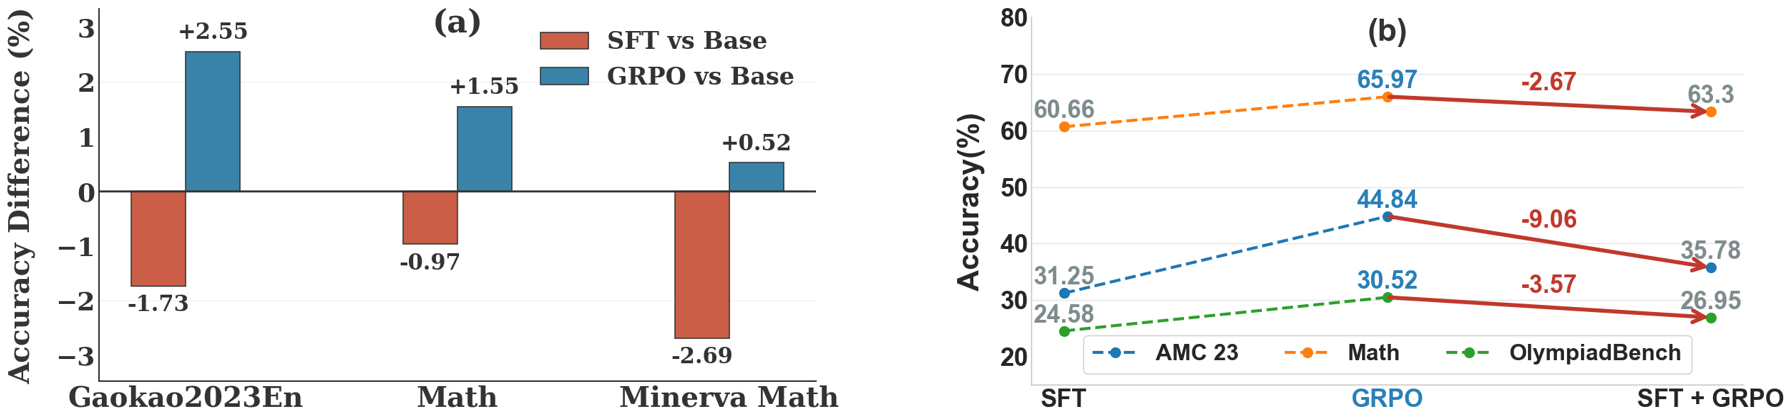
\includegraphics[width=1\linewidth]{GFT/Figure/intro.png}
    \caption{Performance of Qwen2.5-Math-1.5B on Numina-Math. (a) Accuracy changes relative to the base model: SFT consistently degrades performance, highlighting catastrophic forgetting. (b) Accuracy across different training pipelines: the SFT+GRPO pipeline exhibits poor synergy, underperforming GRPO alone.}
    \label{fig:intro}
\end{figure*}


% To address this gap, we present a principled theoretical analysis from the perspective of training dynamics.
% We show that SFT can be interpreted as a special case of reinforcement learning.
% Specifically, SFT implicitly corresponds to a policy gradient method with an extremely sparse reward function $r(x,y)=\mathbb{I}[y=y^{*}]$, which forces the model to imitate a single expert trajectory and leads to insufficient exploration and entropy collapse.
% Moreover, its gradient updates are weighted by an inverse probability coefficient $w(y|x)=1/\pi_{\theta}(y|x)$.
% When the model encounters valid but unfamiliar expert tokens, this coefficient can grow excessively large, triggering gradient explosion and driving the model toward mechanical memorization and overfitting.
% Together, sparse implicit rewards and unstable inverse-probability weighting constitute the fundamental causes of SFT's limited generalization ability.

To investigate the root causes of these challenges, we present a principled theoretical analysis from the perspective of training dynamics. We demonstrate that SFT can be interpreted as a special case of reinforcement learning, but one that suffers from two fundamental flaws: (1) It is constrained by \textbf{single-path dependency}, where the implicit reward $r(x,y)=\mathbb{I}[y=y^{*}]$ restricts the learning signal to the exact expert trajectory, leading to \textbf{insufficient exploration} and \textbf{entropy collapse}. (2) It is vulnerable to \textbf{gradient explosion} during optimization. Since the gradient updates are scaled by an \textbf{unstable importance weight} $w(y|x)=1/\pi_{\theta}(y|x)$ (the reciprocal of the token probability), valid but unfamiliar expert tokens cause this weight to grow excessively large, triggering \textbf{gradient explosion} and driving the model toward \textbf{mechanical memorization} and \textbf{overfitting}. Together, these factors constitute the mathematical explanation for SFT's limited generalization ability.

Motivated by these theoretical insights, we propose \textbf{Group Fine-Tuning (GFT)}, a unified post-training paradigm designed to directly mitigate these intrinsic deficiencies.
GFT introduces two key mechanisms.
\emph{Group Advantage Learning} overcomes SFT's single-path dependency by creating a diverse response group for each query, combining model-generated samples, expert demonstrations, and teacher outputs.
% By computing statistically normalized relative advantages within each group, instead of enforcing a rigid imitation of expert data, GFT employs group-relative advantage weighting. 
By evaluating candidates according to their normalized within-group advantages, rather than rigidly imitating expert data, this approach produces learning signals that are comparable across diverse responses, thereby preserving essential exploration during early post-training.
\emph{Dynamic Coefficient Rectification} stabilizes optimization while preserving learning capacity through a clipping-like adaptive weighting scheme.
By applying a dynamic threshold $\tau$ to the \textbf{importance weight} $w(y|x)$, this mechanism suppresses gradient explosion for extreme samples while \textbf{preserving the effective gradient} for moderately low-probability tokens, enabling efficient injection of new knowledge into models.

%%%% 实验结论
% The empirical validity of our approach is substantiated by comprehensive evaluations using the Qwen2.5-Math models~\citep{yang2024qwen2} on six demanding mathematical reasoning benchmarks—AMC23~\citep{amc2023dataset}, College Math~\citep{hendrycks2020measuring}, Gaokao~\citep{zhang2023evaluating}, Math~\citep{hendrycks2021measuring}, Minerva Math~\citep{lewkowycz2022solving}, and TabMWP\citep{lu2022dynamic}. GFT consistently delivers substantial performance gains, significantly surpassing not only standard SFT and GRPO baselines but also recent state-of-the-art variants, including DFT~\citep{wu2025generalization}, ASFT~\citep{zhu2025anchored}, and PSFT~\citep{zhu2025proximal}. Furthermore, our analysis highlights the superior synergy between GFT and Reinforcement Learning (RL). By preserving policy diversity and mitigating the rigidity induced by standard SFT, GFT serves as a more effective initialization, enabling subsequent RL stages to overcome the ``synergy dilemma'' and achieve significantly higher performance ceilings.

We systematically evaluated GFT across multiple model families and math-reasoning benchmarks. Compared with standard SFT, strong SFT variants such as DFT \cite{wu2025generalization} and ASFT \cite{zhu2025anchored}, RL baselines such as GRPO, and component-wise ablations, GFT consistently outperforms all baselines on both standard and competition-level tasks with substantially higher data efficiency. To further probe the post-training “synergy dilemma,” we use GFT as the initialization for subsequent RL and contrast it with the conventional “SFT→RL” pipeline; GFT provides a stronger cold start and more stable optimization, thereby significantly raising the attainable performance ceiling of RL. Finally, evaluations of catastrophic forgetting and output diversity show that GFT markedly mitigates the severe forgetting typical of SFT while achieving a practical unification of improved precision and preserved exploration.

\noindent\textbf{Our main contributions include:}
\newline\textbullet\ From a training-dynamics perspective, we identify two causes of SFT’s weak generalization:
(i) inherent single-path dependency, where each context is supervised by a single expert demonstration; and
(ii) gradient explosion, which promotes mechanical memorization and catastrophic forgetting.
\newline\textbullet\ We propose \textbf{GFT}, unifying unbiased group advantages and token-wise update stabilization into a single-stage post-training procedure by combining group advantage learning with dynamic importance weight rectification.
\newline\textbullet\ Extensive experiments across multiple benchmarks show that GFT consistently outperforms standard SFT and strong SFT-based baselines, validating GFT as a foundational post-training paradigm for LLMs.




% Our main contributions include:
% \begin{itemize}
% \item First, from a training-dynamics perspective, we identify two causes of SFT’s weak generalization: (i) inherent single-path dependency, where each context is supervised by a single expert demonstration; and (ii) gradient explosion, which promotes mechanical memorization and consequent catastrophic forgetting.
% \item Second, we propose GFT, which unifies unbiased group
% advantages and token-wise update stabilization into a single-stage post-training procedure by combining group advantage learning with dynamic importance weight rectification.
% \item Third, extensive experiments across multiple benchmarks demonstrate that GFT consistently outperforms standard SFT and strong SFT-based baselines, validating its effectiveness as a new foundational paradigm for post-training large language models.
% \end{itemize}


% With the rapid development of Large Language Models (LLMs) and Multimodal Models (VLMs), stimulating the inference and generalization abilities of models in complex tasks has become a core research focus. Currently, Supervised Fine-Tuning (SFT) and Reinforcement Learning (RL) form the standard paradigm for the post-training stage: typically, SFT is first used to perform a ``cold start'' through expert demonstration data, endowing the model with specific instruction-following abilities and domain knowledge; subsequently, RL (such as PPO or GRPO) is employed to further optimize inference logic through exploration and feedback. However, although both methods possess distinct strengths, existing serial or simple combination strategies are revealing their limitations in the pursuit of higher-order intelligence. Achieving strong generalization ability while ensuring the efficient injection of new knowledge remains an open challenge.

% Current post-training paradigms suffer from intrinsic limitations and a significant ``synergy dilemma.'' While SFT efficiently injects knowledge~\citep{zhou2024lima}, it inherently relies on behavioral cloning, often leading to ``mechanical imitation'' and poor performance on out-of-distribution (OOD) data~\citep{chu2025sft,huan2025math,swamy2025roads}. Conversely, RL excels at exploring robust strategies but struggles to acquire complex knowledge from scratch, making it highly dependent on initialization~\citep{mandlekar2021matters, chen2025empirical}. Crucially, when trained sequentially, SFT-induced overfitting creates a rigid policy that constrains the exploration space required for the subsequent RL stage~\citep{chen2025sft}. Furthermore, the fundamental divergence in their reasoning patterns—where SFT tends toward verbose, structured reasoning while RL favors conciseness—implies that traditional pipelines often achieve only a trade-off or compromise, rather than fundamentally fusing their respective advantages~\citep{chen2025synergy}.

% \textbf{To resolve this synergy dilemma, we must scrutinize the fundamental \textit{misalignment} between the two paradigms, which manifests in two distinct aspects:}

% \textbf{First, the misalignment in data distribution: Single-Path Dependency vs. Diverse Exploration.} 
% SFT typically relies on behavioral cloning of static, single-path expert demonstrations. This limits the model to mechanically memorizing specific human-provided trajectories, effectively creating a ``narrow-minded'' policy. In contrast, RL algorithms (like GRPO) require the model to learn from a broader distribution of self-generated rollouts to distinguish superior strategies. The \textit{single-path dependency} of SFT fails to provide this necessary exploration space, creating a distributional shift that hinders the seamless transition to the subsequent RL stage.

% \textbf{Second, the misalignment in optimization mechanism: Unconstrained Fitting vs. Stable Evolution.} 
% The optimization of SFT is aggressive and unconstrained: it enforces a hard constraint to maximize the likelihood of target tokens, regardless of how ``surprising'' or out-of-distribution they are. This often results in drastic gradient updates that force the model to memorize outliers or noise (overfitting). Conversely, RL methods typically employ ``trust region'' constraints (e.g., ratio clipping) to ensure the policy evolves gradually without deviating too far from the reference. SFT's lack of such a ``safety brake'' leads to catastrophic forgetting of general logic, making the model ill-conditioned for the delicate optimization of RL.

% To address these misalignments and achieve both effective knowledge learning and robust generalization, we propose a unified framework: \textbf{Group-based Fine-Tuning (GFT).} Our method is grounded in the theoretical analysis of Dynamic Fine-Tuning (DFT)~\citep{wu2025generalization}, where we view the SFT gradient as a special type of policy gradient. From this perspective, we identify that the implicit reward structure of SFT suffers from two main theoretical limitations that correspond to the challenges above. First, its implicit reward $r(x,y)=\mathbf{1}[y=y^{*}]$ is extremely sparse, forcing the model to mimic a single path (Entropy Collapse). Second, its gradient uses a coefficient $w(y|x) = 1/\pi_{\theta}(y|x)$ that is inversely proportional to the prediction probability. When the model encounters unfamiliar expert demonstrations, this coefficient becomes excessively large, leading to ``gradient explosion'' and overfitting.

% Based on this analysis, our proposed \textbf{GFT} paradigm is designed to directly address these intrinsic flaws:
% \begin{enumerate}
%     \item To address the \textbf{reward sparsity problem}, GFT introduces a GRPO-like \textit{Group Advantage Learning} mechanism. By constructing a response group with diverse trajectories and calculating standardized contrastive feedback, GFT breaks SFT's single-path dependency, maintaining the exploration capability required for generalization.
%     \item To address the \textbf{coefficient explosion problem}, GFT proposes a \textit{Threshold-based Dynamic Coefficient Rectification (DCR)} mechanism. This mechanism preserves the efficient SFT injection capability for ``new knowledge tokens'' while dynamically suppressing the gradient explosion from ``extreme tokens'' using a probability threshold $\tau$.
% \end{enumerate}

% This theoretically-driven modification transforms SFT's unstable, overfit-prone update process into a novel training paradigm that can efficiently inject new knowledge while achieving stable generalization. We conducted extensive experiments on multiple benchmark datasets. Our results show that the GFT paradigm not only significantly outperforms the traditional SFT baseline but also consistently surpasses advanced SFT improvement methods. Our main contributions include:
% \begin{itemize}
%     \item We theoretically analyze the root causes of SFT's weak generalization, revealing its dual flaws of gradient coefficient explosion and implicit reward sparsity.
%     \item We propose GFT, a unified post-training paradigm that utilizes group advantage learning and dynamic coefficient rectification to simultaneously mitigate SFT's overfitting while preserving efficient knowledge injection.
%     \item We demonstrate the effectiveness and robustness of the GFT framework through extensive experiments, proving its capability to serve as a generic bridge that harmonizes the conflict between supervised cloning and reinforcement exploration.
% \end{itemize}

% 注意:目前related work是参考的DFT论文的，后续会根据篇幅进行修改与调整
% \input{Anonymous/Main/Section/related_work}

% \section{Related Work}





% 注意:目前related work是参考的DFT论文的，后续会根据篇幅进行修改与调整

% \section{Method}

% \subsection{Preliminaries}
% \label{sec:preliminaries}

% % 确保在导言区引用了 amsmath 和 amssymb
% % \usepackage{amsmath}
% % \usepackage{amssymb}

% \paragraph{Gradient Representation of Supervised Fine-Tuning (SFT)}
% In Supervised Fine-Tuning (SFT), the model $\pi_{\theta}$ is trained on an expert demonstration dataset $\mathcal{D}=\{(x,y^{*})\}$. The objective is to minimize the negative log-likelihood. The gradient of the parameters, denoted as $\nabla_{\theta}\mathcal{L}_{SFT}(\theta)$, is expressed as follows:
% \begin{equation}
%     % 0.92 表示缩小为原来的 92%
%     \scalebox{0.88}{%
%         $\displaystyle
%         \nabla_{\theta}\mathcal{L}_{SFT}(\theta) = \mathbb{E}_{(x,y^{*})\sim\mathcal{D}}[-\nabla_{\theta}\log \pi_{\theta}(y^{*}|x)]
%         $%
%     }
%     \label{eq:sft_grad}
% \end{equation}

% \paragraph{Gradient Representation of Reinforcement Learning (RL)}
% In Reinforcement Learning (RL), the policy $\pi_{\theta}$ generates responses by interacting with the environment and is optimized based on a reward function $r(x,y)$. The policy gradient at the sentence level, denoted as $\nabla_{\theta}J(\theta)$, is expressed as:
% \begin{equation}
%     \scalebox{0.88}{%
%     $\displaystyle
%     \nabla_{\theta}J(\theta)=\mathbb{E}_{x\sim\mathcal{D}_{x},y\sim\pi_{\theta}(\cdot|x)}[\nabla_{\theta}log~\pi_{\theta}(y|x)r(x,y)]
%     $%
%     }
%     \label{eq:rl_grad}
% \end{equation}

% \paragraph{Transforming SFT Gradient to RL Form}
% To theoretically analyze the generalization limitations of SFT, we refer to the method proposed in DFT and rewrite the SFT gradient (Eq.\ref{eq:sft_grad}) into the paradigm of the RL policy gradient (Eq.\ref{eq:rl_grad}). 

% The SFT gradient is originally an expectation calculated under the fixed expert demonstration distribution $\mathcal{D}$. We transform it into an on-policy expectation under the model's own policy distribution $\pi_{\theta}$ by introducing the Importance Sampling identity. The derivation is as follows:
% % 使用 align 环境处理长公式，& 用于对齐，\\ 用于换行
% % \nonumber 用于不给中间步骤编号，节省版面混乱度
% \begin{align}
%     \nabla_{\theta}&\mathcal{L}_{SFT}(\theta) \nonumber \\
%     &= \mathbb{E}_{(x,y^{*})\sim\mathcal{D}}[-\nabla_{\theta}\log \pi_{\theta}(y^{*}|x)] \nonumber \\
%     &= \mathbb{E}_{x\sim\mathcal{D}_{x}, y \sim \delta(\cdot|y^{*})}[-\nabla_{\theta}\log \pi_{\theta}(y|x)] \nonumber \\
%     &= \mathbb{E}_{\substack{x\sim\mathcal{D}_{x} \\ y \sim \pi_{\theta}(\cdot|x)}} \left[ \frac{P_{expert}(y|x)}{Q(y|x)} [-\nabla_{\theta}\log \pi_{\theta}(y|x)] \right] \nonumber \\
%     % 暴力压缩最后一行
%     &= \mathbb{E}_{\substack{x\sim\mathcal{D}_{x} \\ y \sim \pi_{\theta}(\cdot|x)}} \left[ \frac{P_{expert}(y|x)}{Q(y|x)} [-\nabla_{\theta}\log \pi_{\theta}(y|x)] \right] \nonumber \\
%     % 使用 multlined 将最后一行拆分为两行
%     &= \begin{multlined}[t]
%         \mathbb{E}_{\substack{x\sim\mathcal{D}_{x} \\ y \sim \pi_{\theta}(\cdot|x)}} \bigg[ \frac{\delta(y - y^*)}{\pi_{\theta}(y|x)} \\
%         \cdot [-\nabla_{\theta}\log \pi_{\theta}(y|x)] \bigg]
%       \end{multlined}
% \end{align}

% Since $\delta(y - y^*)$ is 1 only when $y = y^*$ and 0 otherwise ($y \ne y^*$), we can replace $\delta(y - y^*)$ with an equivalent indicator function $\cdot{1}[y = y^*]$. Rearranging the expression, we obtain:
% \begin{equation}
% \begin{split}
%     \nabla_{\theta}\mathcal{L}_{SFT}(\theta) &= \\
%     -\mathbb{E}_{\substack{x\sim\mathcal{D}_{x} \\ y\sim\pi_{\theta}(\cdot|x)}} & \bigg[ \frac{1}{\pi_{\theta}(y|x)} \nabla_{\theta}\log \pi_{\theta}(y|x) \\
%     & \quad \cdot \mathbf{1}[y = y^*] \bigg]
% \end{split}
% \label{eq:sft_final_form}
% \end{equation}


% \subsection{Theoretical Analysis}
% \label{sec:root_cause_analysis}

% As shown in Section \ref{sec:preliminaries}, SFT functions as a special case of RL policy gradient (Eq. \ref{eq:sft_final_form}). Based on this perspective, we identify two key factors that limit the generalization of SFT:

% \subsubsection{Gradient Variance and Coefficient Explosion}
% The SFT gradient is scaled by an inverse weight $w(y|x) = 1/\pi_{\theta}(y|x)$. When the model assigns low probability to expert tokens, this weight becomes excessively large, triggering \textbf{gradient explosion}. This instability compels the model to memorize outliers in expert trajectories, significantly degrading its ability to generalize to unseen data.

% \subsubsection{Sparsity of Implicit Rewards}
% SFT relies on a sparse, binary reward: $r(x,y)=\mathbf{1}[y=y^{*}]$. This signal only validates the exact ground truth, forcing the model to ignore the quality of other potential paths. However, robust generalization requires more than just memorizing the \textbf{unique correct} answer. The model should also learn to compare different candidates and understand why some paths are inferior. SFT lacks this \textbf{contrastive feedback}, restricting the model's capability to explore and generalize beyond the training distribution.

% \subsection{Group-based Fine-Tuning}
% \label{sec:gft}

% Based on the analysis in Section \ref{sec:root_cause_analysis}, we propose \textbf{Group-based Fine-Tuning (GFT)}. GFT aims to address both the reward sparsity and coefficient explosion of SFT within a unified framework. The method consists of two tightly integrated components: (1) Multi-path learning with group advantages to provide dense contrastive feedback; and (2) Threshold-based dynamic coefficient rectification to stabilize gradients while preserving the injection of new knowledge.

% \subsubsection{Multi-path Learning with Group Advantage}
% To overcome the limitation of learning from a single ``perfect'' path in SFT, we construct a response group $\mathcal{G}_x = \{y_1, y_2, ..., y_K\}$ for each query $x$. This group consists of two parts:
% \begin{itemize}
%     \item \textbf{Demonstration Trajectories ($y_{demo}$):} This includes the ground truth from the dataset, as well as responses distilled from stronger external models. Crucially, these distilled answers may contain imperfections or errors. This diversity allows the model to expose to a broader, more realistic distribution of answers, rather than just a single expert solution.
%     \item \textbf{Sampled Trajectories ($y_{sample}$):} We sample $K-1$ additional responses from the current model policy: $y_{sample} \sim \pi_{\theta}(\cdot|x)$.
% \end{itemize}

% \subsubsection{Group Reward and Advantage}
% For every response $y_k$ in $\mathcal{G}_x$ (whether demonstration or sampled), we compute a scalar reward $R(y_k)$ based on its match with the ground truth. To provide stable and discriminative contrastive signals, we compute the advantage $A(y_k)$ using group normalization (consistent with GRPO):
% \begin{equation}
%     A(y_k) = \frac{R(y_k) - \bar{R}(\mathcal{G}_x)}{\sigma_R(\mathcal{G}_x) + \epsilon}
%     \label{eq:advantage}
% \end{equation}
% where $\bar{R}(\mathcal{G}_x)$ is the mean reward and $\sigma_R(\mathcal{G}_x)$ is the standard deviation within the group. $\epsilon$ is a small constant (e.g., $10^{-8}$) for numerical stability.

% A positive $A(y_k)$ indicates the path is better than average, while a negative value implies it is worse. This standardized signal allows the model to explicitly ``penalize'' poor paths and ``reward'' high-quality ones, effectively solving the implicit reward sparsity of SFT.

% \subsubsection{Threshold-based Dynamic Coefficient Rectification}

% To address the coefficient explosion discussed in Section \ref{sec:root_cause_analysis}, we design a Dynamic Coefficient Rectification mechanism. We recognize that the SFT coefficient $1/\pi_{\theta}$ is a double-edged sword:
% \begin{itemize}
%     \item \textbf{Harmful ``Extreme Tokens'':} When $\pi_{\theta}$ is extremely low, the coefficient becomes huge, causing gradient explosion and overfitting.
%     \item \textbf{Beneficial ``New Knowledge Tokens'':} When $\pi_{\theta}$ is low but reasonable, a larger coefficient helps the model effectively learn new, unmastered knowledge.
% \end{itemize}

% Simply removing the coefficient for all tokens (as in DFT) may hinder the learning of new knowledge. Therefore, we introduce a probability threshold $\tau$ and a dynamic rectification factor $\mathcal{C}(\pi_t)$. The rectified loss for each token is:
% \begin{equation}
%     \mathcal{L}_{\text{token}}(\theta, y_t) = \mathcal{C}(\pi_t) \cdot [-\log \pi_t]
% \end{equation}
% where $\pi_t = \pi_{\theta}(y_t|y_{<t}, x)$. The rectification factor $\mathcal{C}(\pi_t)$ is defined as:
% \begin{equation}
%     \mathcal{C}(\pi_t) = 
%     \begin{cases} 
%         \text{sg}(\pi_t) & \text{if } \pi_t < \tau \\ 
%         1 & \text{if } \pi_t \ge \tau 
%     \end{cases}
%     \label{eq:rectification_factor}
% \end{equation}
% Here, $\text{sg}(\cdot)$ denotes the stop-gradient operator.

% \begin{itemize}
%     \item \textbf{Case 1: $\pi_t < \tau$ (Extreme Token).} The factor becomes $\text{sg}(\pi_t)$. The gradient is scaled by $\pi_t$, effectively canceling the $1/\pi_t$ term and preventing explosion.
%     \item \textbf{Case 2: $\pi_t \ge \tau$ (New/Mastered Knowledge).} The factor is $1$. The loss reverts to standard SFT loss, preserving the strong signal needed for knowledge injection.
% \end{itemize}

% \subsubsection{Final GFT Loss}
% The final objective function combines both components. We use the normalized advantage $A(y_k)$ as a weight for the total rectified trajectory loss:
% \begin{equation}
%     % 压缩到栏宽的 95%，确保编号能放得下
%     \resizebox{0.89\hsize}{!}{$
%         \displaystyle
%         \mathcal{L}_{\text{GFT}}(\theta) = \mathbb{E}_{x \sim \mathcal{D}_x, \mathcal{G}_x} \left[ \sum_{y_k \in \mathcal{G}_x} \text{sg}(A(y_k)) \cdot \mathcal{L}_{\text{traj}}(\theta, y_k) \right]
%     $}
%     \label{eq:gft_final}
% \end{equation}
% where $\mathcal{L}_{\text{traj}}(\theta, y_k) = \sum_{t=1}^{|y_k|} \mathcal{C}(\pi_{\theta}(y_{k,t}|y_{k,<t}, x)) \cdot [-\log \pi_{\theta}(y_{k,t}|...)]$ is the sum of rectified token losses.

% Through this design, GFT achieves: (1) dense, standardized contrastive rewards for all trajectories; and (2) dynamic suppression of noise from extreme tokens while ensuring effective learning of new knowledge.




\section{Preliminaries}\label{sec:preliminaries}

In SFT learning process, the policy model $\pi_{\theta}$ is trained to imitate expert demonstrations. Given a expert dataset $\mathcal{D}=\{(x,y^{*})\}$, the gradient of the SFT objective with model parameters $\theta$ is
\begin{equation}
    \nabla_{\theta}\mathcal{L}_{\mathrm{SFT}}
    =
    \mathbb{E}_{\mathcal{D}}
    \big[
    -\nabla_{\theta}\log \pi_{\theta}(y^{*}\mid x)
    \big].
    \label{eq:sft_grad}
\end{equation}

This gradient increases the likelihood of the expert-provided response and does not explicitly consider alternative outputs. However, in RL training process, the output $y$ is generated by the current model $\pi_{\theta}(\cdot\mid x)$ itself. The reward $r(x, y)$ is then computed for this model-generated sample. The policy gradient takes the form
\begin{equation}
    \nabla_{\theta}\mathcal{L}_{\mathrm{RL}}
    =
    \mathbb{E}_{x,y}
    \big[
    -\nabla_{\theta}\log \pi_{\theta}(y\mid x)\, r(x,y)
    \big].
    \label{eq:rl_grad}
\end{equation}

Notably, SFT can be viewed as a special case of RL. Specifically, if we interpret the SFT objective as maximizing a sparse reward that only provides non-zero feedback for the expert trajectory, its gradient can be rewritten as an on-policy expectation over $\pi_{\theta}$ via importance sampling. This equivalent formulation is:
\begin{equation}
\begin{split}
    \nabla_{\theta}\mathcal{L}
    =
    -\mathbb{E}_{x, y}
    \Big[
    \frac{\mathbb{I}[y=y^{*}]}{\pi_{\theta}(y\mid x)}
    \nabla_{\theta}\log \pi_{\theta}(y\mid x)
    \Big],
\end{split}
\label{eq:sft_final_form}
\end{equation}
where the indicator $\mathbb{I}[y=y^{*}]$ serves as a sparse reward that assigns a unit signal only when the sampled output exactly matches the expert demonstration, and zero otherwise. The term $1/\pi_{\theta}(y\mid x)$ corresponds to an importance weight that corrects for sampling from the current policy $\pi_{\theta}$ instead of the expert distribution.
The detailed derivation is provided in Appendix \ref{sec:proof}.

Eq.~\eqref{eq:sft_final_form} exposes two intrinsic limitations of SFT from an RL perspective. First, \textbf{single-path dependency} arises as the sparse reward confines learning to a single expert trajectory, offering no comparative feedback over alternatives. Second, \textbf{gradient explosion} occurs because the importance weight $1/\pi_{\theta}(y\mid x)$ grows excessively when the expert action probability is small, leading to highly unstable optimization behavior.




% In SFT, the model $\pi_{\theta}$ is trained on an expert demonstration dataset $\mathcal{D}=\{(x,y^{*})\}$. The gradient of the negative log-likelihood loss is expressed as:
% \begin{equation}
%     \scalebox{0.9}{%
%         $\displaystyle
%         \nabla_{\theta}\mathcal{L}_{SFT}(\theta) = \mathbb{E}_{(x,y^{*})\sim\mathcal{D}}[-\nabla_{\theta}\log \pi_{\theta}(y^{*}|x)]
%         $%
%     }
%     \label{eq:sft_grad}
% \end{equation}

% In RL, the policy $\pi_{\theta}$ generates responses by interacting with the environment and is optimized based on a reward function $r(x,y)$. The policy gradient is:
% \begin{equation}
%     \scalebox{0.88}{%
%     $\displaystyle
%     \nabla_{\theta}J(\theta)=\mathbb{E}_{x\sim\mathcal{D}_{x},y\sim\pi_{\theta}(\cdot|x)}[\nabla_{\theta}log~\pi_{\theta}(y|x)r(x,y)]
%     $%
%     }
%     \label{eq:rl_grad}
% \end{equation}

% To analyze the generalization limitations of SFT, we transform the SFT gradient into an on-policy RL formulation (detailed derivation is provided in the \textbf{Appendix}). The equivalent gradient form is:
% \begin{equation}
% \begin{split}
%     \nabla_{\theta}\mathcal{L}_{SFT}(\theta) &= \\
%     -\mathbb{E}_{\substack{x\sim\mathcal{D}_{x} \\ y\sim\pi_{\theta}(\cdot|x)}} & \bigg[ \underbrace{\frac{1}{\pi_{\theta}(y|x)}}_{\text{Importance Weight}} \nabla_{\theta}\log \pi_{\theta}(y|x) \\
%     & \quad \cdot \underbrace{\mathbf{1}[y = y^*]}_{\text{Sparse Reward}} \bigg]
% \end{split}
% \label{eq:sft_final_form}
% \end{equation}

% Eq. (\ref{eq:sft_final_form}) reveals two critical flaws limiting SFT's generalization:
% \begin{itemize}
%     \item \textbf{Single-Path Dependency:} The indicator term $\mathbf{1}[y=y^*]$ restricts the model to mimicking a single expert trajectory, ignoring all other potential reasoning paths. This lack of contrastive feedback between ``better'' and ``worse'' answers prevents the model from distinguishing robust logic from rote memorization.
    
%     \item \textbf{Coefficient Explosion:} The weight $1/\pi_{\theta}$ becomes excessively large when the model is unfamiliar with the target tokens (low probability). This causes unstable gradient updates and forces the model to memorize outliers.
% \end{itemize}

\section{Method: Group Fine Tuning}

\begin{figure*}[h]
    \centering
    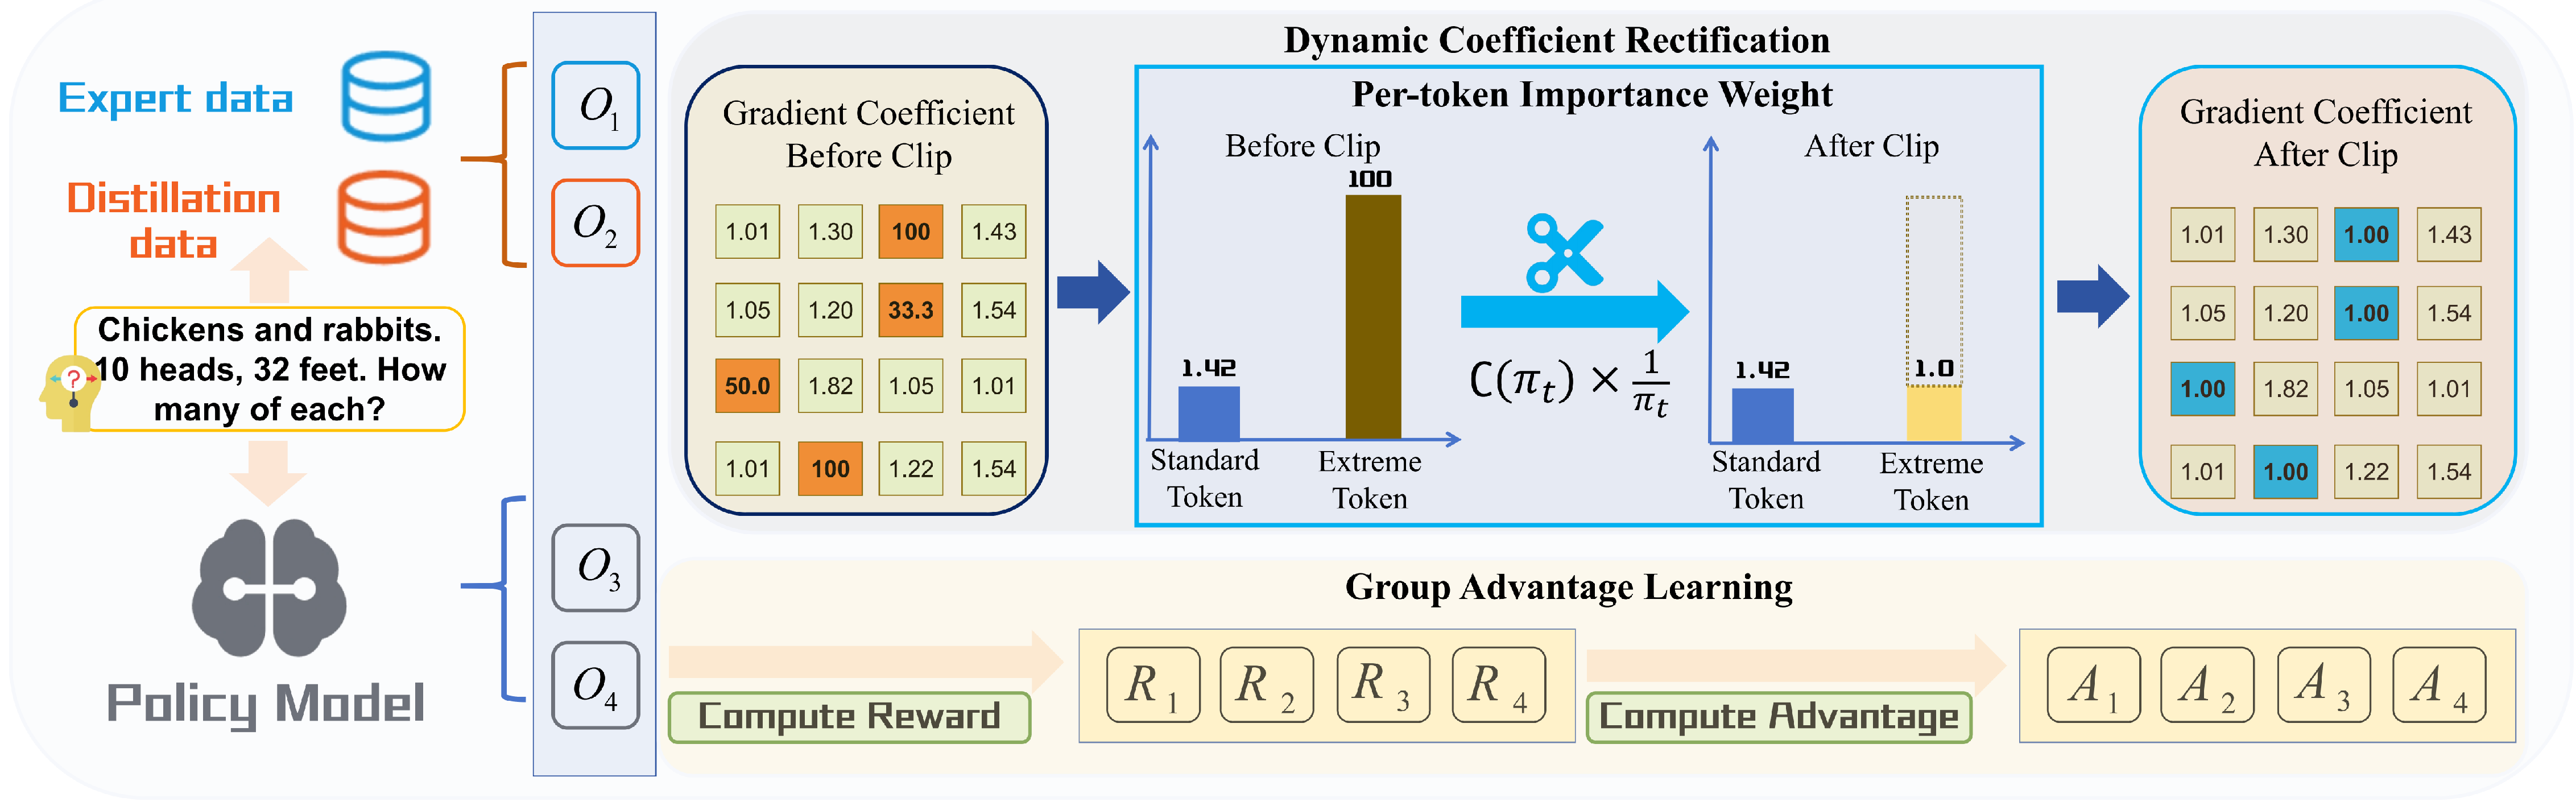
\includegraphics[width=1\linewidth]{GFT/Figure/method2.pdf}
    \caption{GFT comprises two components: (1) \textit{Group Advantage Learning}, which computes standardized relative advantages ($A_k$) from hybrid response groups (expert demonstrations, teacher outputs, and rollout samples); and (2) \textit{Dynamic Coefficient Rectification}, which bounds importance weights via per-token gradient clipping.}
    \label{fig:overview}
\end{figure*}

To address the intrinsic limitations of SFT identified in Eq.~\eqref{eq:sft_final_form}, we propose two complementary mechanisms.
\textbf{Group Advantage Learning} (GAL) constructs a group of multiple candidate trajectories for one query and evaluates each trajectory based on rule-consistent rewards, allowing the model to learn from diverse reasoning paths rather than treating only expert demonstrations as correct.
\textbf{Dynamic Coefficient Rectification} (DCR) stabilizes training by clipping the weight $1/\pi_{\theta}(y\mid x)$ for extremely low-probability tokens, preventing gradient explosion while preserving the original gradient for standard tokens to ensure efficient knowledge injection.
% \textbf{Dynamic Coefficient Rectification} (DCR) stabilizes training by clipping the weight $1/\pi_{\theta}(y\mid x)$ for extremely low-probability tokens, preventing gradient explosion while retaining sufficient update strength for informative low-confidence predictions.


\subsection{Group Advantage Learning}

To move beyond the limitations of single-path dependency, we expand the standard SFT dataset into a comprehensive hybrid response group $\mathcal{G}x = {y_1, ..., y_K}$ for each query $x$. This group strategically integrates three complementary data sources: \textbf{Expert Demonstrations} ($y_{\text{exp}}$) that provide ground truth to guarantee a valid optimization direction always exists; \textbf{Teacher Distillations} ($y_{\text{demo}}$) from other powerful models, introducing diverse reasoning paradigms to break single-path dependency; and \textbf{Self-Generated Samples} ($y_{\text{sample}}$) obtained from the model's own rollouts, offering on-policy feedback to rectify intrinsic errors while reinforcing successful self-exploration. This design maintains high flexibility, allowing the composition to adapt based on data availability and training objectives. To effectively utilize the strengths of each data source within a unified learning framework, we assign a scalar reward $R(y_k)$ to each response in group $\mathcal{G}_x$, then compute a standardized advantage score:
\begin{equation}
A(y_k) = \frac{R(y_k) - \mu(\mathcal{G}_x)}{\sigma_R(\mathcal{G}_x) + \epsilon},
\label{eq:advantage}
\end{equation}
where \(\bar{R}(\mathcal{G}_x)\) and \(\sigma_R(\mathcal{G}_x)\) denote the mean and standard deviation of rewards within the group, and \(\epsilon > 0\) is a small constant that ensures numerical stability. This normalization centers and scales the rewards, creating a \textbf{relative, contrastive signal} within the group. Consequently, the reward mechanism guides the model to discern and prioritize high-quality responses, effectively unifying imitation, distillation, and self-improvement within a single, stable objective.
% Guided by the theoretical analysis in Eq. \ref{eq:sft_final_form}, we attribute the limited generalization of SFT to two intrinsic limitations. First, the \textbf{Single-Path Depedency} restricts the model to mimicking a unique expert trajectory, preventing it from learning diverse reasoning paradigms. Second, SFT operates via a \textbf{Non-contrastive Mechanism}: it trains solely on the correct expert path, effectively ignoring all other generated trajectories. To systematically resolve these issues, we propose \textbf{Group Advantage Learning}, which proceeds in two steps:

% To expand the learning scope beyond a single expert trajectory, we construct a hybrid response group $\mathcal{G}_x = \{y_1, ..., y_K\}$ for each query. This group integrates trajectories from two complementary sources: \textbf{Teacher Distillations} ($y_{demo}$) to introduce diverse reasoning paradigms, and \textbf{Self-Generated Samples} ($y_{sample}$) to expose the model's actual performance boundaries. By aggregating these multiple perspectives into a single group, we force the model to learn a broader solution space rather than overfitting to a rigid template.

% To overcome the blindness of SFT's non-contrastive mechanism, we must enable the model to distinguish between the varying qualities within this mixed group. We quantify the relative quality of each response by computing the standardized advantage $A(y_k)$:
% \begin{equation}
%     A(y_k) = \frac{R(y_k) - \bar{R}(\mathcal{G}_x)}{\sigma_R(\mathcal{G}_x) + \epsilon}
%     \label{eq:advantage}
% \end{equation}
% This formulation transforms the learning objective from simple imitation to \textbf{comparative discrimination}. It encourages the model to align with high-advantage trajectories (superior strategies) while explicitly penalizing low-advantage ones (errors or inferior paths), thereby fostering robust generalization.


%%%%%%%%%%%%%%3.1.2 DCR %%%%%%%%%%%%%%%%%%%%%%%%%%%%%%

\subsection{Dynamic Coefficient Rectification}

The theoretical analysis in Eq.~\eqref{eq:sft_final_form} reveals that the inverse probability term $1/\pi_{\theta}$ introduces an inherent instability into the SFT-style optimization.
In practice, this instability arises in two common and complementary scenarios.
First, when the model increases its exploration by rolling out uncertain or diverse responses, the predicted token probabilities $\pi_t$ can become small, causing the corresponding update coefficients to grow excessively large.
Second, even when fitting expert demonstrations or teacher-distilled responses, the model may initially assign low probability to valid but unfamiliar tokens, which similarly amplifies the inverse weighting term. Inspired by the gradient clipping technique prevalent in RL, we propose a simple rectification function to stabilize the training:
\begin{equation}\label{eq:rectification_factor}
        \mathcal{C}(\pi_t) = 
        \begin{cases} 
            \text{sg}(\pi_t) & \text{if } \pi_t < \tau\\ 
            1 & \text{if } \pi_t \ge \tau
        \end{cases}
\end{equation}

Here, $\tau$ is a confidence threshold, and $\text{sg}(\cdot)$ denotes the stop-gradient operator. This design actively suppresses the explosive term $1/\pi_t$ for low-confidence tokens ($\pi_t < \tau$) by using $\text{sg}(\pi_t)$ to yield a bounded effective coefficient, while leaving the gradient unchanged for confident predictions ($\pi_t \ge \tau$). This ensures stable updates during exploration and preserves full learning strength for knowledge transfer, effectively resolving the instability inherent in the SFT objective.

% The theoretical analysis in Eq. \ref{eq:sft_final_form} identifies the inverse weight $1/\pi_{\theta}$ as a \textbf{double-edged sword}. In practice, for a specific token probability $\pi_t$, this coefficient dictates the update strength:

% When the model encounters valid new knowledge, $\pi_t$ is naturally low but within a reasonable range. The resulting \textbf{substantial} coefficient $1/\pi_t$ provides an \textbf{amplified} gradient signal, facilitating rapid learning and adaptation. However, for "extreme tokens" (outliers or noise) where $\pi_t \approx 0$, this coefficient becomes excessively large. This triggers gradient explosion, compelling the model to overfit to specific data points rather than learning general patterns.


% To balance stability and plasticity, we propose \textbf{Dynamic Coefficient Rectification (DCR)}. We define $\pi_t = \pi_{\theta}(y_t|y_{<t}, x)$ as the prediction probability for the current token and introduce a threshold $\tau$ to dynamically rectify the loss:

% \begin{equation}\label{eq:rectification_factor}
%         \mathcal{C}(\pi_t) = 
%         \begin{cases} 
%             \text{sg}(\pi_t) & \text{if } \pi_t < \tau ~~ \text{\small (Suppress Explosion)} \\ 
%             1 & \text{if } \pi_t \ge \tau ~~ \text{\small (Inject Knowledge)} 
%         \end{cases}
% \end{equation}

% Here, $\text{sg}(\cdot)$ denotes the stop-gradient operator. When $\pi_t < \tau$, the factor $\text{sg}(\pi_t)$ neutralizes the explosive $1/\pi_t$ term ($1/\pi_t \cdot \pi_t = 1$) to ensure stability; otherwise, it remains $1$, preserving the necessary gradient strength for knowledge injection.

\subsection{Final GFT Objective}
Combining Group Advantage Learning and Dynamic Coefficient Rectification, we derive the final training objective in its gradient form.
% For each input $x$, responses are sampled from the constructed group $\mathcal{G}_x$, and the policy is updated using advantage-weighted, rectified gradients:
{\small
\begin{equation}\label{eq:gft_gradient}
\nabla_{\theta}\mathcal{L}
=
\mathbb{E}_{y_k {\in} \mathcal{G}_x}
\Big[
A(y_k)
\frac{\mathcal{C}(\pi)}{\pi_{\theta}(y_k|x)}
\nabla\!\log \pi_{\theta}(y_k|x)
\Big].
\end{equation}
}
Eq.~\eqref{eq:gft_gradient} presents the sequence-level gradient of GFT; the corresponding token-level formulation and loss definition are provided in Appendix \ref{sec:formulation}.
This gradient directly resolves the two intrinsic limitations of SFT: group-wise advantage weighting introduces contrastive supervision across multiple trajectories, while dynamic coefficient rectification bounds the update magnitude for low-probability tokens to prevent gradient explosion.


% Integrating both components, the final GFT loss is defined as the expected loss over the group, weighted by the advantage:
% \begin{equation}
% \begin{split}
%     \mathcal{L}_{\text{GFT}}(\theta) = \mathbb{E}_{x \sim \mathcal{D}_x, \mathcal{G}_x} \bigg[ & \sum_{y_k \in \mathcal{G}_x} \text{sg}(A(y_k)) \cdot {} \\
%     & \sum_{t=1}^{|y_k|} \mathcal{C}(\pi_{t}) [-\log \pi_{t}] \bigg]
% \end{split}
% \label{eq:gft_final}
% \end{equation}
% This formulation allows GFT to achieve the ``best of both worlds'': the dense, explorative feedback of RL and the efficient instruction-following capability of SFT, without the instability of standard weighting.

%%%%%%%%%%%%%%%%%%%%%%%%%%%%%%%%%%%%%%%%%%%%%%%%%%%%%%%%%%%%%%%%%%%%%%%%%%%%%%%%%%%%%%%%%%%%%%%%%%%%%%%%
% 实验
%%%%%%%%%%%%%%%%%%%%%%%%%%%%%%%%%%%%%%%%%%%%%%%%%%%%%%%%%%%%%%%%%%%%%%%%%%%%%%%%%%%%%%%%%%%%%%%%%%%%%%%%

\section{Experiments}
\subsection{Experimental Setup}
\label{sec:experimental_setup}

\paragraph{Baselines and Models}
We compare GFT against a diverse set of paradigms, ranging from standard SFT and its recent stabilized variants—DFT~\citep{wu2025generalization}, ASFT~\citep{zhu2025anchored}, and PSFT~\citep{zhu2025proximal}—to the reinforcement learning baseline GRPO. Following DFT~\citep{wu2025generalization}, we evaluate five models covering diverse sizes, types and architectures: Qwen2.5-Math (1.5B, 7B)~\citep{yang2024qwen2}, LLaMA-3 (3.2-3B, 3.1-8B)~\citep{dubey2024llama}, and DeepSeekMath-7B-Base~\citep{shao2024deepseekmath}.

\paragraph{Training Settings}
Following prior works~\citep{wu2025generalization,zhu2025anchored,ming2025one,zhou2025variational}, we utilize the NuminaMath CoT dataset~\citep{numina_math_datasets}, selected for its extensive diversity ranging from high school exercises to international olympiads. For GFT, we construct a hybrid response group of size $K=8$ per query, comprising 1 expert demonstration, 3 teacher distillations from Qwen2.5-Math-72B, and 4 self-generated samples. Similarly, the GRPO baseline is configured to generate 8 outputs per query. To align total training volume, GFT and GRPO utilize a 10k subset (8 trajectories per query), whereas single-trajectory baselines (e.g., SFT) use 100k samples. See Appendix~\ref{sec:eval_settings} for evaluation details.

% \paragraph{Evaluation Settings}
% We conduct evaluations on a broad suite of 11 benchmarks: AMC23~\citep{amc2023dataset}, College Math~\citep{hendrycks2020measuring}, Gaokao~\citep{zhang2023evaluating}, Math~\citep{hendrycks2021measuring}, Minerva Math~\citep{lewkowycz2022solving}, TabMWP~\citep{lu2022dynamic}, OlympiadBench~\citep{he-etal-2024-olympiadbench}, Mmlu Stem~\citep{hendrycks2020measuring}, Sat Math~\citep{zhong2024agieval}, Mawps~\citep{koncel2016mawps}, and Svamp~\citep{patel2021nlp}. These benchmarks are carefully selected to cover a wide spectrum of difficulty levels and reasoning types, ensuring a holistic assessment of the model's capabilities. We report the average Pass@1 accuracy across 16 decoding runs (Pass@16 Average) with a sampling temperature of 0.5 and a maximum generation length of 4096 tokens.


\subsection{Main Results}
\label{sec:main_results}

\begin{table*}[!t]
    \centering
    \small 
    \caption{Main results on seven math benchmarks. \textbf{SFT(mix)} indicates that the dataset is a mixture of expert datasets and distilled teacher datasets, while \textbf{GFT(no mix)} represents using only expert datasets without distilled data. \textbf{Bold} and \colorbox{blue!10}{blue} denote the best intra-group and overall performance, respectively. Overall, GFT achieves the best average performance across diverse model scales.}
    \label{tab:main_results}
      
    \resizebox{\textwidth}{!}{%
        \setlength{\tabcolsep}{3pt} 
        \renewcommand{\arraystretch}{1.2} 
        \begin{tabular}{llcccccc}
            \toprule
            \textbf{Model} & \textbf{Method} & \textbf{AMC23} & \textbf{College Math} & \textbf{Gaokao2023En} & \textbf{Math} & \textbf{Minerva Math} & \textbf{TabMWP} \\
            \midrule
              
            % 第一组: Qwen2.5-Math-1.5B
            \multirow{9}{*}{\textbf{Qwen2.5-Math-1.5B}} 
            & Base Model & 30.16 & 24.30 & 34.81 & 46.54 & 10.51 & 24.55 \\
            & + SFT & 31.25 (+1.09) & 36.45 (+12.15) & 48.86 (+14.05) & 60.66 (+14.12) & 23.99 (+13.48) & 79.34 (+54.79) \\
            & + SFT(mix) & 32.70 (+2.54) & 36.35 (+12.05) & 50.82 (+16.01) & 60.41 (+13.87) & 25.76 (+15.25) & 80.15 (+55.60) \\
            & + GRPO & 44.84 (+14.68) & 35.58 (+11.28) & 51.80 (+16.99) & 65.97 (+19.43) & 21.17 (+10.66) & 76.94 (+52.39) \\
            & + ASFT & 43.12 (+12.96) & 29.40 (+5.10) & 47.99 (+13.18) & 60.35 (+13.81) & 15.55 (+5.04) & 65.06 (+40.51) \\
            & + PSFT & 31.56 (+1.40) & 33.77 (+9.47) & 47.66 (+12.85) & 59.51 (+12.97) & 19.13 (+8.62) & 71.61 (+47.06) \\
            & + DFT & 36.40 (+6.24) & 38.76 (+14.46) & 52.75 (+17.94) & 64.35 (+17.81) & 23.75 (+13.24) & 82.08 (+57.53) \\
            \cmidrule(l){2-8}
            & \textbf{+ GFT(no mix)} & 42.18 (+12.02) & 39.37 (+15.07) & 55.59 (+20.78) & 68.13 (+21.59) & 27.77 (+17.26) & 82.21 (+57.66) \\
            & \textbf{+ GFT (Ours)} & \cellcolor{blue!10}\textbf{46.09 (+15.93)} & \cellcolor{blue!10}\textbf{40.51 (+16.21)} & \cellcolor{blue!10}\textbf{58.32 (+23.51)} & \cellcolor{blue!10}\textbf{70.50 (+23.96)} & \cellcolor{blue!10}\textbf{28.93 (+18.42)} & \cellcolor{blue!10}\textbf{85.24 (+60.69)} \\
            \midrule
              
            % 第二组: Qwen2.5-Math-7B
            \multirow{9}{*}{\textbf{Qwen2.5-Math-7B}} 
            & Base Model & 42.66 & 34.31 & 49.50 & 59.10 & 19.20 & 85.32 \\
            & + SFT & 41.88 (-0.78) & 38.31 (+4.00) & 54.69 (+5.19) & 67.16 (+8.06) & 31.82 (+12.62) & 87.67 (+2.35) \\
            & + SFT(mix) & 43.06 (+0.40) & 39.47 (+5.16) & 56.83 (+7.33) & 69.63 (+10.53) & 32.45 (+13.25) & 88.93 (+3.61) \\
            & + GRPO & 55.63 (+12.97) & 38.65 (+4.34) & 61.63 (+12.13) & 73.29 (+14.19) & 32.60 (+13.40) & 91.18 (+5.86) \\
            & + ASFT & 52.81 (+10.15) & \cellcolor{blue!10}\textbf{40.76 (+6.45)} & 61.55 (+12.05) & 74.31 (+15.21) & 32.47 (+13.27) & 89.37 (+4.05) \\
            & + PSFT & 41.56 (-1.10) & 38.05 (+3.74) & 56.74 (+7.24) & 67.30 (+8.20) & 34.86 (+15.66) & 83.55 (-1.77) \\
            & + DFT & 51.09 (+8.43) & 39.31 (+5.00) & 57.46 (+7.96) & 70.42 (+11.32) & 35.31 (+16.11) & 86.94 (+1.62) \\
            \cmidrule(l){2-8}
            & \textbf{+ GFT(no mix)} & 53.21 (+10.55) & 38.74 (+4.43) & 61.72 (+12.22) & 74.78 (+15.68) & 34.22 (+15.02) & 92.90 (+7.58) \\
            & \textbf{+ GFT (Ours)} & \cellcolor{blue!10}\textbf{56.09 (+13.43)} & 40.24 (+5.93) & \cellcolor{blue!10}\textbf{63.47 (+13.97)} & \cellcolor{blue!10}\textbf{77.31 (+18.21)} & \cellcolor{blue!10}\textbf{39.86 (+20.66)} & \cellcolor{blue!10}\textbf{93.81 (+8.49)} \\
            \midrule
              
            % 第三组: DeepSeekMath-7B
            \multirow{9}{*}{\textbf{DeepSeekMath-7B-Instruct}} 
            & Base Model & 16.09 & 27.56 & 38.00 & 42.73 & 19.44 & 75.70 \\
            & + SFT & 20.93 (+4.84) & 31.53 (+3.97) & 43.13 (+5.13) & 46.51 (+3.78) & 18.71 (-0.73) & 79.30 (+3.60) \\
            & + SFT(mix) & 21.57 (+5.48) & \cellcolor{blue!10}\textbf{32.28 (+4.72)} & 42.43 (+4.43) & \cellcolor{blue!10}\textbf{47.52 (+4.79)} & 20.00 (+0.56) & 78.97 (+3.27) \\
            & + GRPO & 16.72 (+0.63) & 27.59 (+0.03) & 42.18 (+4.18) & 43.39 (+0.66) & 19.39 (-0.05) & 77.74 (+2.04) \\
            & + ASFT & 15.52 (-0.57) & 28.40 (+0.84) & 39.03 (+1.03) & 44.51 (+1.78) & 15.38 (-4.06) & 77.42 (+1.72) \\
            & + PSFT & \cellcolor{blue!10}\textbf{25.78 (+9.69)} & 30.05 (+2.49) & 43.84 (+5.84) & 45.36 (+2.63) & 18.20 (-1.24) & 78.91 (+3.21) \\
            & + DFT & 24.37 (+8.28) & 30.68 (+3.12) & 43.90 (+5.90) & 47.01 (+4.28) & 19.00 (-0.44) & 79.88 (+4.18) \\
            \cmidrule(l){2-8}
            & \textbf{+ GFT(no mix)} & 18.43 (+2.34) & 30.90 (+3.34) & 42.56 (+4.56) & 45.14 (+2.41) & 19.38 (-0.06) & 77.97 (+2.27) \\
            & \textbf{+ GFT (Ours)} & 23.12 (+7.03) & 30.98 (+3.42) & \cellcolor{blue!10}\textbf{48.15 (+10.15)} & 44.79 (+2.06) & \cellcolor{blue!10}\textbf{20.42 (+0.98)} & \cellcolor{blue!10}\textbf{80.08 (+4.38)} \\
            \midrule
              
            % 第四组: LLaMA-3.2-3B
            \multirow{9}{*}{\textbf{LLaMA-3.2-3B-Instruct}} 
            & Base Model & 23.78 & 25.40 & 38.06 & 44.63 & 14.83 & 69.12 \\
            & + SFT & 19.53 (-4.25) & 26.12 (+0.72) & 36.33 (-1.73) & 43.66 (-0.97) & 12.14 (-2.69) & 68.40 (-0.72) \\
            & + SFT(mix) & 21.09 (-2.69) & 27.88 (+2.48) & 37.76 (-0.30) & 45.68 (+1.05) & 14.15 (-0.68) & 70.00 (+0.88) \\
            & + GRPO & 23.25 (-0.53) & 28.01 (+2.61) & 40.61 (+2.55) & 46.18 (+1.55) & 18.44 (+3.61) & 67.53 (-1.59) \\
            & + ASFT & 18.44 (-5.34) & 26.13 (+0.73) & 37.49 (-0.57) & 43.65 (-0.98) & 11.38 (-3.45) & 66.64 (-2.48) \\
            & + PSFT & 24.37 (+0.59) & 28.94 (+3.54) & 40.73 (+2.67) & 47.43 (+2.80) & 15.41 (+0.58) & 70.91 (+1.79) \\
            & + DFT & 14.21 (-9.57) & 26.63 (+1.23) & 35.13 (-2.93) & 41.45 (-3.18) & 9.58 (-5.25) & 67.39 (-1.73) \\
            \cmidrule(l){2-8}
            & \textbf{+ GFT(no mix)} & \cellcolor{blue!10}\textbf{27.66 (+3.88)} & \cellcolor{blue!10}\textbf{31.14 (+5.74)} & \cellcolor{blue!10}\textbf{43.88 (+5.82)} & \cellcolor{blue!10}\textbf{51.71 (+7.08)} & \cellcolor{blue!10}\textbf{21.29 (+6.46)} & 72.87 (+3.75) \\
            & \textbf{+ GFT (Ours)} & 27.50 (+3.72) & 30.15 (+4.75) & 43.25 (+5.19) & 49.60 (+4.97) & 18.84 (+4.01) & \cellcolor{blue!10}\textbf{72.93 (+3.81)} \\
            \bottomrule
        \end{tabular}%
    }
\end{table*}

% For the 1.5B model, GFT delivers substantial improvements. Notably, on the challenging Minerva Math benchmark, GFT achieves a score of 32.19, which is more than \textbf{1.5 times higher} than the mainstream GRPO baseline (20.94). Surprisingly, the performance of the 1.5B model trained with GFT even surpasses that of the larger 7B base models trained with standard methods. This indicates that GFT effectively activates the model's potential and achieves high data efficiency.Similar trends are observed on larger models such as Qwen2.5-Math-7B, DeepSeekMath-7B, and LLaMA-3.1-8B. GFT consistently outperforms other baselines on both simple tasks (like Math500) and hard competition-level tasks (like AIME24 and Olympiad Bench). While standard SFT sometimes struggles with overfitting on small datasets, GFT maintains robust generalization. This demonstrates that our proposed dual-mechanism—group advantage learning and dynamic coefficient rectification—works universally well across different model scales and families.
Based on Table~\ref{tab:main_results}, GFT demonstrates strong data efficiency under a reduced training budget: with only 10k training examples, it matches or even surpasses a range of baselines trained with 100k examples. Crucially, mixing in distillation data yields only marginal changes for both SFT and GFT (i.e., \textit{SFT(mix)} $\approx$ \textit{SFT} and \textit{GFT(no mix)} $\approx$ \textit{GFT}), indicating that the gains are not primarily driven by additional distilled traces but by the proposed training mechanism. Notably, for smaller heterogeneous models like Llama-3.2-3B, \textsc{GFT (no mix)} surpasses mixing strategies, implying they are less robust to the distribution mismatch from the teacher's distinct reasoning patterns. This superior performance is consistently observed across different model scales and model families, suggesting that the improvements are largely model-agnostic. In terms of the performance profile, GFT yields more uniform gains: whereas some methods exhibit uneven improvements or trade-offs across benchmarks, GFT tends to improve performance across diverse evaluations simultaneously. This suggests that GFT is not merely adapting to a specific question format, but is more reliably improving the quality of the underlying reasoning process. Meanwhile, GRPO can be close to GFT because both are largely driven by GAL that converts sparse (often near-binary) rewards into lower-variance, more informative signals; moreover, under our training setting without explicit KL regularization, GRPO's implicit update stabilization can partially overlap with the effect of our DCR, effectively thereby narrowing down the apparent gap between them.

% These results align with GFT’s dual-mechanism. Group advantage learning converts binary rewards into lower-variance, more informative advantage signals via within-group comparisons, thereby increasing the amount of effective learning signal per sample. Dynamic coefficient rectification, under a training setting without explicit KL regularization, adaptively controls update strength to mitigate training overshoot and distributional drift, allowing gains to translate more stably across benchmarks. 
% Together, these two components enable GFT to deliver robust and transferable improvements in the low-data regime.

\subsection{Ablation Studies}
\label{sec:ablation}

We validate the contributions of GAL and DCR via ablations on Qwen2.5-Math-1.5B, comparing the full GFT with variants that remove GAL, remove DCR, or remove both (equivalent to standard SFT). We report results on Math, AMC23, and Olympiad Bench to cover increasing difficulty and robustness requirements, and further inspect the optimization behavior of each variant using the learning-dynamics plot in Figure \ref{fig:abl_dynamic}.

\begin{table}[!t]
    \centering
    % 【统一修改】使用 footnotesize，去掉 resizebox
    \footnotesize
    \caption{Ablation on \textbf{Qwen2.5-Math-1.5B}. GAL is important for complex reasoning (e.g., Olympiad) and DCR enhances performance by ensuring optimization stability, their synergy yields optimal results.}
    \label{tab:ablation}
    
    % 【统一修改】紧凑列间距
    \setlength{\tabcolsep}{4pt}
    \renewcommand{\arraystretch}{1.2}
    
    \begin{tabular}{lccc}
        \toprule
        \textbf{Method} & \textbf{AMC23} & \textbf{MATH} & \textbf{Olympiad} \\
        \midrule
        Base Model & 30.16 & 46.54 & 23.39 \\
        \midrule
        GFT w/o (GAL + DCR) & 31.25 & 60.66 & 24.58 \\
        GFT w/o GAL & 35.78 & 63.91 & 26.63 \\
        GFT w/o DCR & 42.81 & 65.97 & 27.82 \\
        \textbf{GFT (Ours)} & \textbf{46.09} & \textbf{70.50} & \textbf{30.52} \\
        \bottomrule
    \end{tabular}
\end{table}

\begin{figure}[!t]
    \centering
    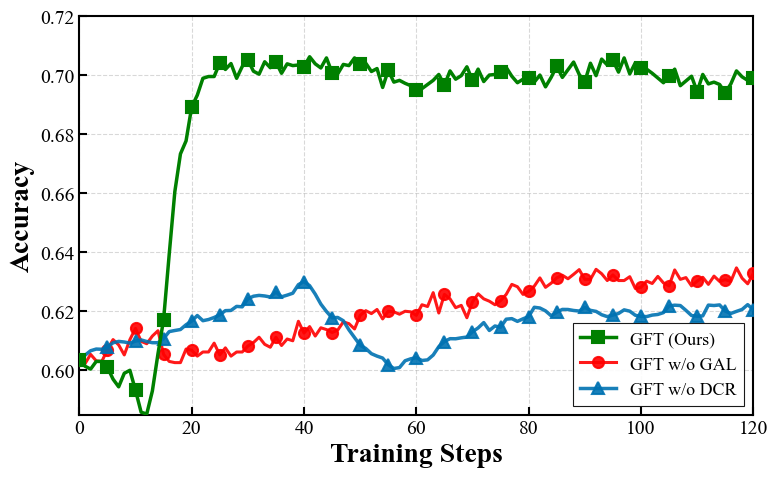
\includegraphics[width=0.5\linewidth]{GFT/Figure/ablation_eval.png}
    \caption{Learning dynamics on MATH-lighteval. Removing DCR causes severe volatility, while removing GAL results in slow convergence and a lower ceiling.}
    \label{fig:abl_dynamic}
\end{figure}

The results in Table \ref{tab:ablation} demonstrate the distinct contributions of each component.
Removing GAL causes the sharpest decline on the hardest benchmark (Olympiad), validating that group-based contrastive feedback is vital for extracting signals in complex reasoning.
In contrast, removing DCR primarily impacts robustness (Minerva), consistent with its role in rectifying gradient explosion.
These performance patterns are further corroborated by the learning dynamics in Figure \ref{fig:abl_dynamic}: the removal of DCR leads to severe training volatility, while removing GAL results in slow, suboptimal convergence.
Ultimately, GFT synergizes both components to ensure efficient and stable optimization.


\subsection{Compatibility with SFT and RL}
\label{sec:compatibility}

% As discussed in Section 1, traditional post-training pipelines (SFT followed by RL) often suffer from a ``synergy dilemma'', where the rigidity of SFT constraints the exploration space for subsequent reinforcement learning. To investigate whether our proposed GFT can mitigate this issue, we conduct a comprehensive compatibility analysis involving SFT, GFT, and GRPO.

% We design a series of sequential training experiments, as outlined in Table \ref{tab:compatibility}. The goal is to evaluate GFT's role in two scenarios: (1) as a superior alternative to SFT for initializing RL (comparing \textit{GFT + GRPO} vs. \textit{SFT + GRPO}), and (2) as an intermediate transition stage to bridge SFT and RL (evaluating \textit{SFT + GFT + GRPO}).

We conduct a sequential-training compatibility study by combining SFT, GFT, and GRPO in different compositions (Figure~\ref{fig:Compatibility_of_GFT}). This design aims to diagnose the \emph{synergy dilemma} in conventional post-training—where SFT may rigidify the policy and narrow the effective exploration manifold for downstream RL—and to evaluate whether GFT can both (i) serve as a stronger initializer for RL and (ii) improve the handoff from SFT to RL.


\begin{figure*}[!t]
    \centering
    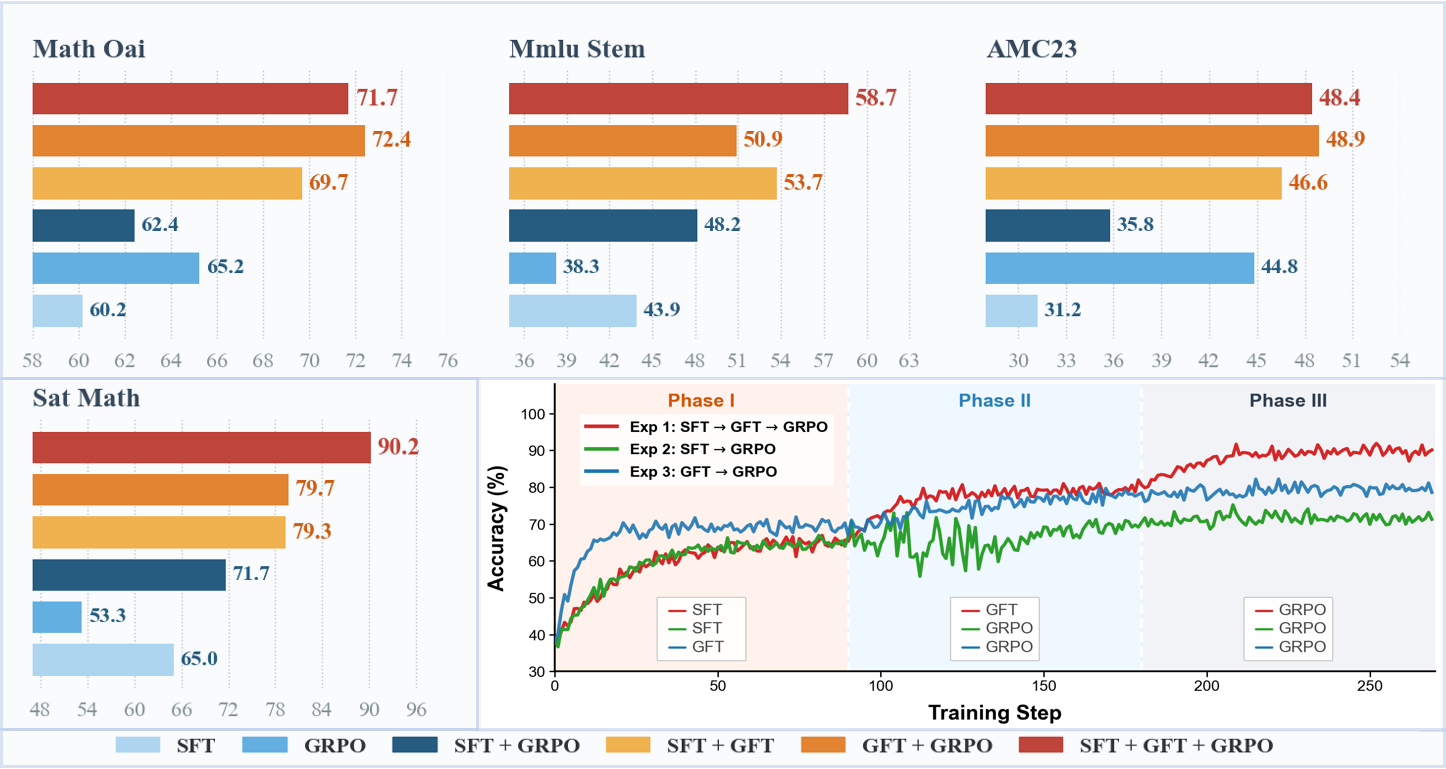
\includegraphics[width=1\linewidth]{GFT/Figure/sft_gft_grpo_merge_2.png}
    \caption{Performance comparison on Qwen2.5-Math-1.5B (Pass@16). Bottom-right: Sat-Math training dynamics. SFT+GFT+GRPO achieves top performance via stable optimization, demonstrating GFT's high compatibility and effective synergy between SFT and GRPO.}
    \label{fig:Compatibility_of_GFT}
\end{figure*}
% \begin{table*}[t]
%     \centering
%     \caption{Compatibility analysis of GFT with SFT and GRPO (RL). ``+'' denotes sequential training (e.g., ``SFT + GRPO'' means training SFT first, then initializing GRPO from the SFT checkpoint). We report Pass@16 Average accuracy on Qwen2.5-Math-1.5B.}
%     \label{tab:compatibility}
%     \resizebox{0.95\textwidth}{!}{%
%         \renewcommand{\arraystretch}{1.3}
%         \setlength{\tabcolsep}{5pt}
%         \begin{tabular}{lcccccc}
%             \toprule
%             \textbf{Training Pipeline} & \textbf{AMC23} & \textbf{AQUA} & \textbf{Math Oai} & \textbf{Minerva Math} & \textbf{Mmlu Stem} & \textbf{Sat Math} \\
%             \midrule
%             Qwen2.5-Math-1.5B (Base) & 30.16 & 23.88 & 46.25 & 10.51 & 19.38 & 15.92 \\
%             \midrule
%             SFT & 31.25 & 41.13 & 60.16 & 23.99 & 43.90 & 65.04 \\
%             GRPO & 44.84 & 19.38 & 65.25 & 21.17 & 38.28 & 53.31 \\
%             SFT + GRPO & 35.78 & 43.60 & 62.41 & 25.79 & 48.17 & 71.68 \\
%             \midrule
%             SFT + GFT & 46.56 & 54.65 & 69.69 & 31.68 & 53.68 & 79.29 \\
%             \textbf{GFT + GRPO} & \textbf{48.91} & 42.12 & \textbf{72.44} & 32.61 & 50.89 & 79.68 \\
%             \textbf{SFT + GFT + GRPO} & 48.43 & \textbf{69.24} & 71.72 & \textbf{33.95} & \textbf{58.71} & \textbf{90.24} \\
%             \bottomrule
%         \end{tabular}%
%     }
% \end{table*}

% \begin{figure}[h]
%     \centering
%     \includegraphics[width=1\linewidth]{GFT/Figure/sft_gft_grpo.png}
%     \caption{Training accuracy curves on the MATH-lighteval}
%     \label{fig:fuse_dynamic}
% \end{figure}

As shown in Figure~\ref{fig:Compatibility_of_GFT}, we design GFT to improve compatibility in two aspects. \textbf{(1) To improve RL exploration,} GAL prevents the cold-start policy from collapsing to a single expert-induced mode and maintains a multi-solution distribution via group-wise relative advantages. This broader support produces more diverse rollouts and stronger advantage signals for GRPO, explaining why \textit{GFT + GRPO} gains more than \textit{SFT + GRPO} on harder benchmarks \cite{li2024preserving}. \textbf{(2) To prevent distribution extremization and preserve exploration,} DCR bounds per-token updates to avoid over-sharpening an SFT-initialized policy. Without this constraint, large steps can quickly drive the policy to a low-entropy, mode-concentrated distribution, reducing rollout diversity and weakening GRPO’s learning signal. By limiting update magnitude, DCR keeps the policy in a higher-entropy regime, matching the smoother dynamics and higher ceiling of \textit{SFT + GFT + GRPO} in Figure~\ref{fig:Compatibility_of_GFT}. \textbf{Notably,} \textit{GFT + GRPO} surpassing \textit{SFT + GRPO} does not mean GFT replaces SFT: SFT provides a reliable initialization point for alignment and formatting, while GFT improves RL compatibility by preserving support and stabilizing updates. Thus, \textit{SFT + GFT + GRPO} works best as a staged pipeline: SFT sets the initialization point, GFT restores exploration capabilities without drifting, and GRPO leverages higher-quality trajectories to reach the top ceiling.




% \paragraph{GFT as a Superior Cold-Start for RL.}
% Comparing the standard pipeline (\textit{SFT + GRPO}) with our proposed pipeline (\textit{GFT + GRPO}), we observe that initializing GRPO with a GFT-tuned model yields significantly better performance. While standard SFT tends to overfit to specific expert paths—creating a ``narrow'' policy that hinders RL exploration [cite: 61]—GFT preserves policy diversity through its Group Advantage mechanism. This allows the subsequent GRPO stage to explore the solution space more efficiently, leading to higher gains on challenging benchmarks like AIME24 and Olympiad Bench.

% \paragraph{GFT as a Bridge between SFT and RL.}
% The results of the three-stage pipeline (\textit{SFT + GFT + GRPO}) are particularly illuminating. When GFT is inserted between SFT and GRPO, it acts as a ``rectifier.'' The intermediate GFT stage effectively mitigates the gradient explosion and rigid patterns introduced by the initial SFT (via the DCR mechanism), reopening the model's learning plasticity. Consequently, the final GRPO stage achieves a higher performance ceiling compared to the direct \textit{SFT + GRPO} baseline. This suggests that GFT is not only a standalone fine-tuning method but also a plug-and-play transition module that enhances the compatibility of existing SFT-RL workflows.

% GFT serves as a generic bridge that harmonizes the conflict between supervised cloning and reinforcement exploration.

\subsection{Catastrophic Forgetting Analysis}
\label{sec:analysis_kl}

\begin{table}[!t]
    \centering
    \footnotesize
   \caption{Performance of ~\textbf{LLaMA-3.2-3B-Instruct} on general reasoning benchmarks. While SFT induces substantial catastrophic forgetting, GFT largely preserves base performance.}
    \label{tab:forgetting_analysis}
    
    \begin{minipage}{0.6\linewidth}
    \centering
    \renewcommand{\arraystretch}{1.1}
    \setlength{\tabcolsep}{2pt}
    
    \begin{tabular*}{\linewidth}{@{\extracolsep{\fill}}lccc}
        \toprule
        \textbf{Method} & \textbf{Mawps} & \textbf{Svamp} & \textbf{Mmlu stem} \\ 
        \midrule
        % Base Model
        Base Model & 96.06 & 86.36 & 41.03 \\
        \midrule
        % SFT
        +SFT & 91.97 (- 4.09) & 78.73 (- 7.63) & 35.05 (-5.98) \\
        
        % GRPO
        +GRPO & 94.60 (-\phantom{0}1.46) & \textbf{88.11 (+\phantom{0}1.75)} & 39.48 (-1.55) \\
        
        % GFT
        +GFT (Ours) & \textbf{95.79 (-\phantom{0}0.27)} & 84.65 (-\phantom{0}1.71) & \textbf{43.89 (+2.86)} \\
        \bottomrule
    \end{tabular*}
    \end{minipage}
\end{table}

\begin{figure}[!t]
    \centering
    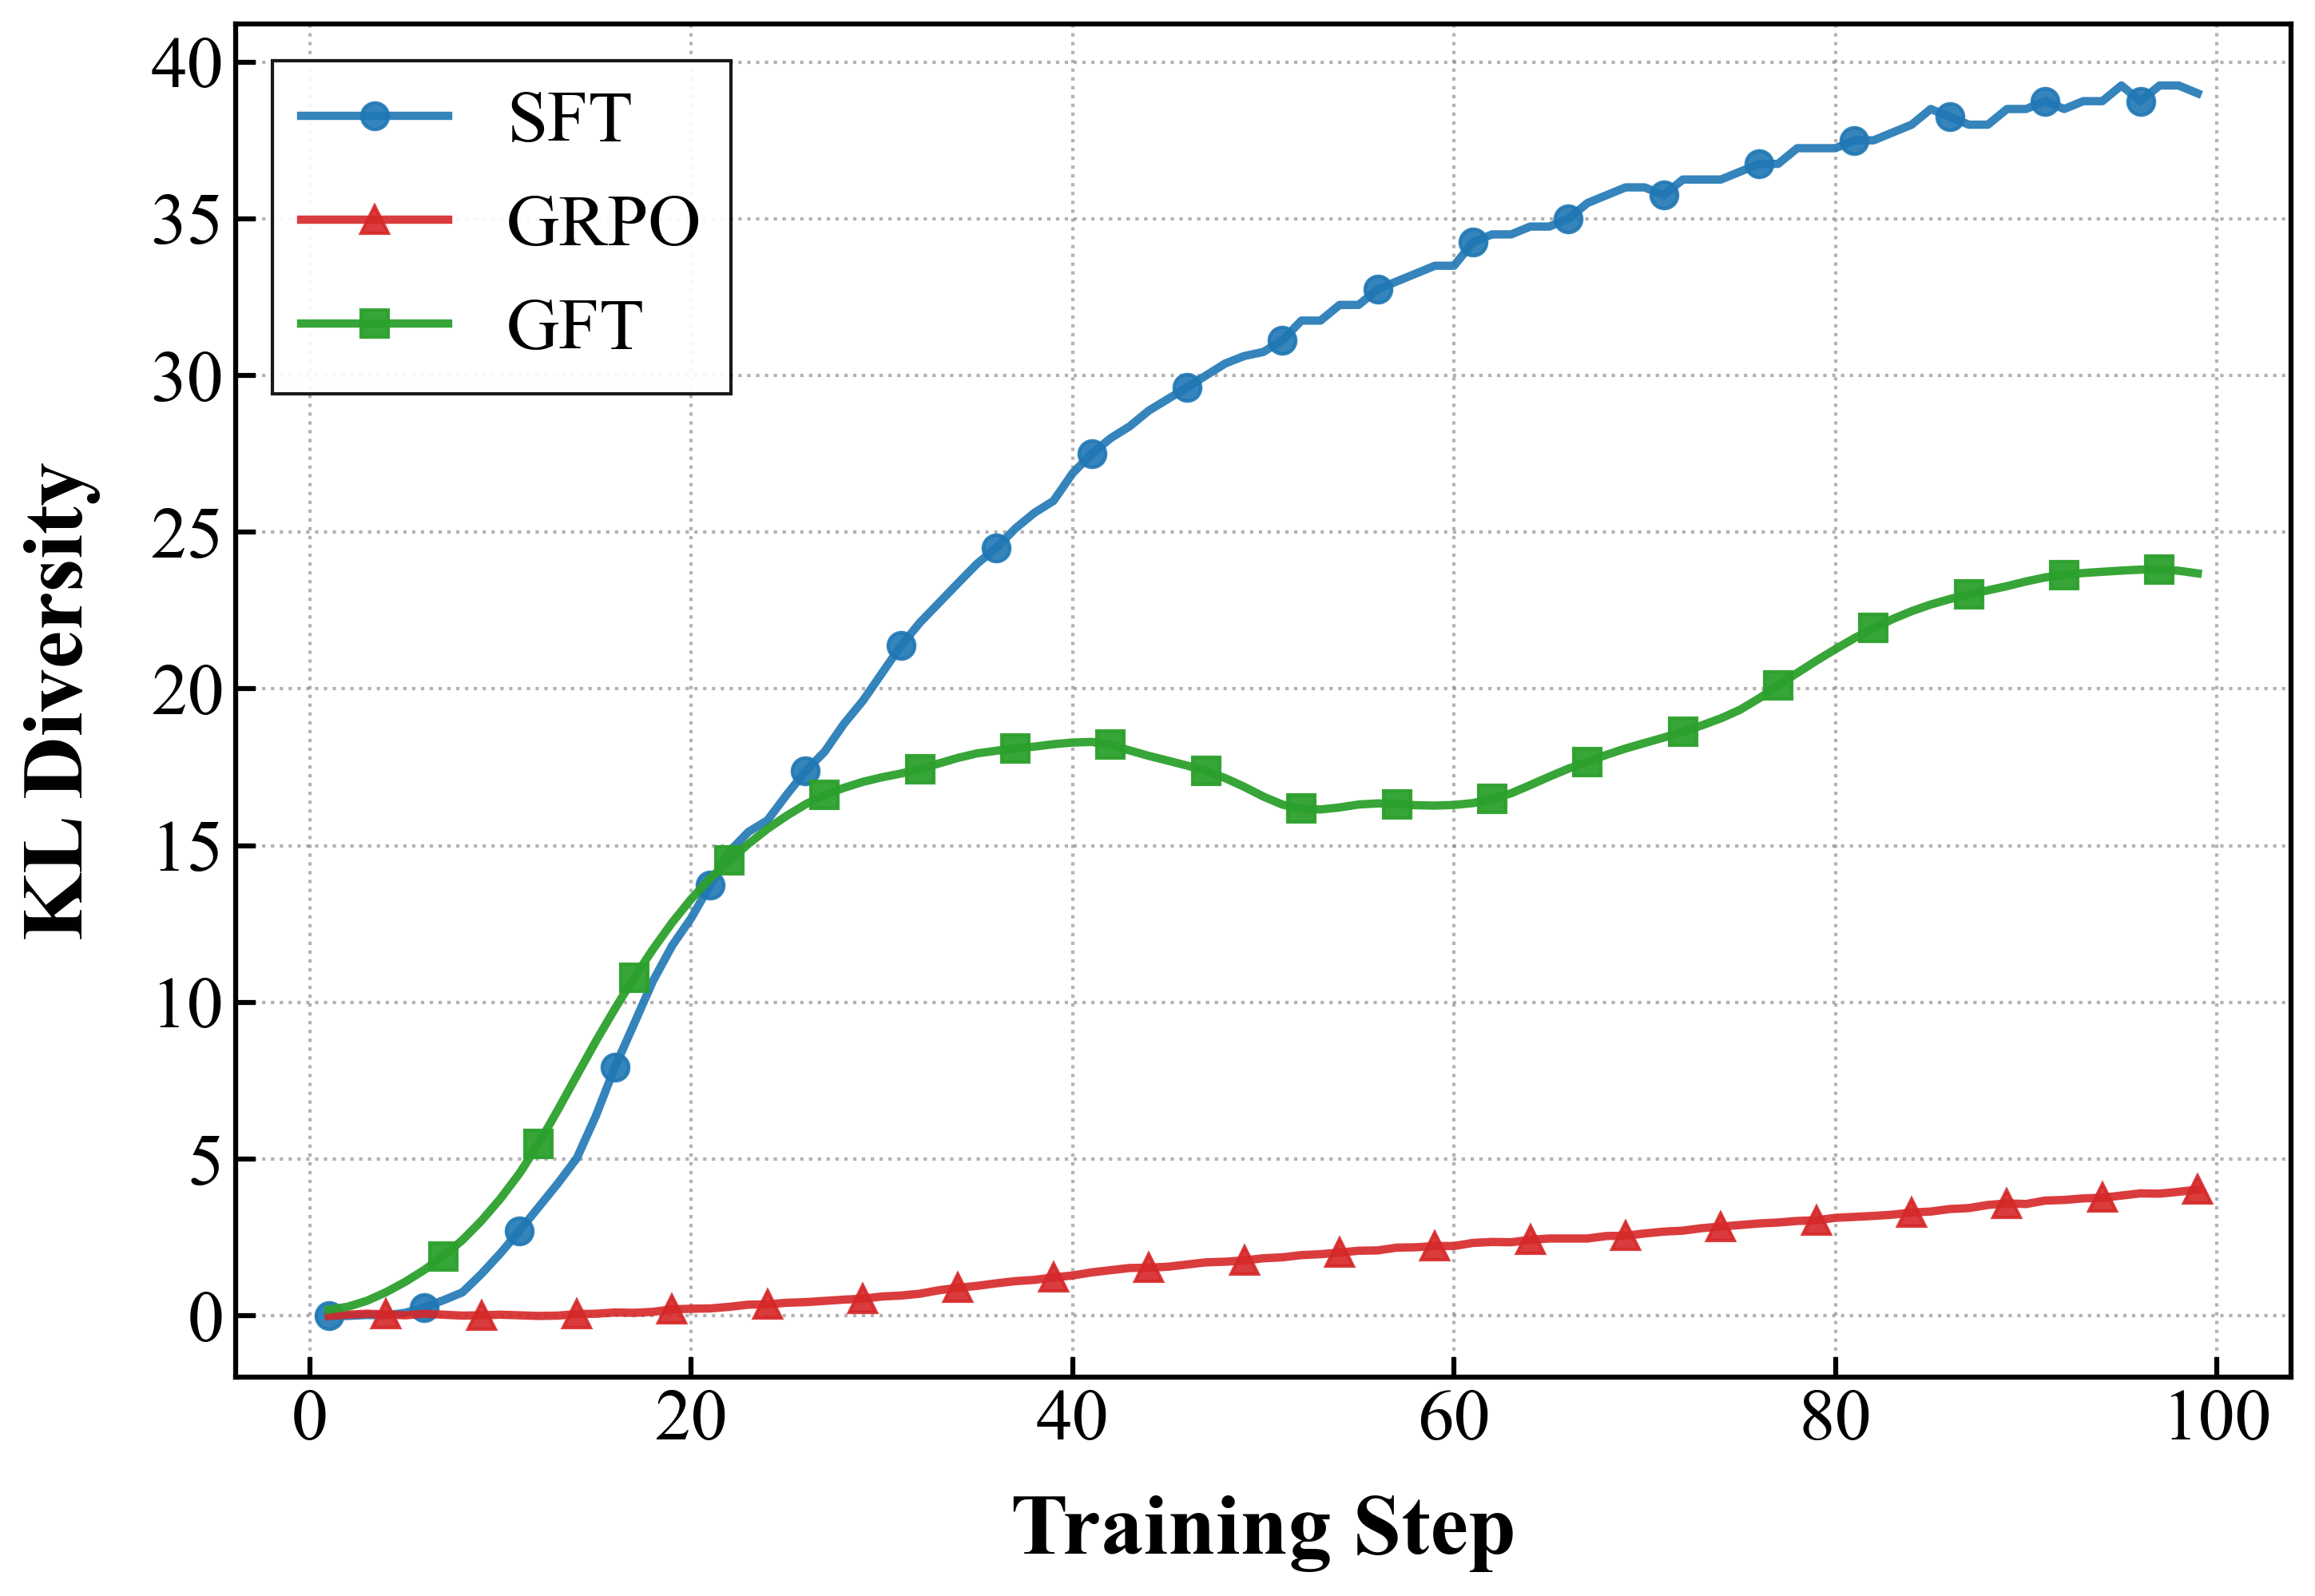
\includegraphics[width=0.5\linewidth]{GFT/Figure/kl.png}
    \caption{KL divergence quantifies distributional drift from the base model. SFT exhibits the highest divergence, while GFT maintains a significantly lower level, effectively mitigating catastrophic forgetting.}
    \label{fig:generation}
\end{figure}

Table~\ref{tab:forgetting_analysis} shows a clear contrast in catastrophic forgetting on general reasoning benchmarks.
After domain training, \textbf{SFT} exhibits substantial degradation on \textsc{MAWPS} and \textsc{SVAMP} and also drops on \textsc{MMLU-STEM}, indicating severe forgetting.
In contrast, \textbf{GRPO} largely preserves the base model's prior capabilities, while \textbf{GFT} not only maintains comparable retention to GRPO but also improves \textsc{MMLU-STEM}.
This ranking is further consistent with Figure~\ref{fig:generation}, where the policy shift of SFT is the most pronounced, whereas GRPO and GFT remain significantly closer to the base policy.



To quantify forgetting more directly, we adopt the approach of~\cite{shenfeld2025rl} and compute the \emph{average KL divergence} between the trained model and the base model on the training dataset. Recent empirical studies further support the correlation between this KL-based drift and forgetting~\citep{chu2025sft, luo2025empirical, ruan2025unveiling}. We therefore use the average KL divergence as a proxy for distributional drift, and hence forgetting.
We analyze the training dynamics of Qwen2.5-Math-1.5B across different methpds.
As shown in Figure~\ref{fig:generation}, all baselines converge to their peak performance approximately at step 100.
At this stage, we observe a distinct contrast: \textbf{SFT} incurs the highest alignment tax with the largest KL divergence, whereas \textbf{GRPO} retains a \emph{KL-minimal} solution; notably, \textbf{GFT} strikes a balance, stabilizing at a low KL level comparable to GRPO.
We attribute this stability to our design: \textbf{GAL} reinforces high-quality output trajectories in a reward-driven manner, avoiding abrupt distributional shifts induced by pure cross-entropy trace fitting; meanwhile, \textbf{DCR} suppresses gradient explosions from ``extreme tokens'' (where $\pi_{\theta}\!\approx\!0$), preventing drastic policy drift.
Together, these components enable efficient knowledge injection while retaining robust general-purpose reasoning.

% To further understand why GFT generalizes better, we analyze different training paradigms through the lens of \emph{training endpoints} and \emph{catastrophic forgetting}. As shown in Figure~\ref{fig:generation}, the parameter endpoint of \textbf{GFT} lies substantially closer to the \textbf{base model} than \textbf{SFT}, and is comparable to GRPO. This observation is consistent with the conclusion in~\cite{shenfeld2025rl}. Figure~\ref{fig:generation} (right) further reveals the forgetting dynamics: while GRPO and GFT maintain relatively stable generalization behavior, \textbf{SFT} shows a pronounced degradation during training, suggesting severe catastrophic forgetting. We corroborate these trends quantitatively by evaluating models on other general reasoning benchmarks before and after training (Table~\ref{tab:forgetting_analysis}), where the ranking is consistent with the figure: SFT forgets markedly, whereas GRPO and GFT largely preserve prior capabilities.

% We attribute GFT's retention to two factors. \textbf{First}, similar to RL, GFT is \emph{reward-driven}: it strengthens the model's ability to produce correct reasoning by reinforcing high-reward trajectories, rather than directly fitting expert traces that can induce abrupt distributional shifts under cross-entropy training. \textbf{Second}, our \textbf{DCR} improves optimization stability by suppressing gradient explosions caused by ``extreme tokens'', thereby preventing drastic policy drift and reducing knowledge forgetting. Together, these properties allow GFT to achieve efficient knowledge injection while retaining robust general-purpose reasoning.

% Table \ref{tab:forgetting_analysis} reveals a stark contrast: while SFT suffers from distinct catastrophic forgetting on general benchmarks, GRPO effectively retains prior knowledge. This aligns with recent findings that SFT tends to drift arbitrarily from the base policy, whereas on-policy RL is biased toward \textit{KL-minimal} solutions~\cite{shenfeld2025rl}. Crucially, GFT matches GRPO's retention capability. This validates that our \textbf{Dynamic Coefficient Rectification (DCR)} effectively mimics this stability. By suppressing the exploding gradients from ``extreme tokens'' (where $\pi_{\theta} \approx 0$), DCR prevents drastic distribution shifts, allowing GFT to achieve the ``best of both worlds'': efficient knowledge injection with robust generalization.

% 修改后的版本:
% To understand GFT's superior generalization, we analyze the training dynamics via KL divergence in Figure~\ref{fig:generation}. \textbf{Distillation} (SFT) exhibits a drastic KL surge ($|kl\_eval| \approx 40$), indicating severe policy drift that correlates with the catastrophic forgetting shown in Table~\ref{tab:forgetting_analysis}, where SFT suffers sharp declines across all tasks (e.g., MAWPS drops from $96.1$ to $82.0$). Conversely, \textbf{GRPO} maintains an extremely low KL ($<5$), reflecting a conservative trajectory. Notably, \textbf{GFT} strikes a critical balance: it allows for moderate distributional shift to facilitate knowledge injection, yet leverages Dynamic Coefficient Rectification (DCR) to curb excessive drift. This controlled plasticity is quantitatively validated in Table~\ref{tab:forgetting_analysis}: unlike SFT, GFT preserves base-level proficiency on standard tasks and uniquely achieves gains on challenging benchmarks like MMLU STEM ($39.0 \rightarrow 43.9$), verifying its ability to enhance reasoning without compromising general capabilities.

% We attribute GFT's retention to two factors. \textbf{First}, being \emph{reward-driven} like RL, it reinforces high-reward trajectories rather than rigidly fitting expert traces, thereby mitigating abrupt distributional shifts. \textbf{Second}, \textbf{DCR} enhances stability by suppressing gradient explosions from ``extreme tokens'', which prevents drastic policy drift and minimizes forgetting. Together, these mechanisms enable GFT to achieve efficient knowledge injection while robustly preserving general-purpose reasoning.


% To further investigate the underlying mechanism of GFT's superior generalization, we analyze the behavior of different training paradigms from the perspective of \textit{training endpoints} and \textit{catastrophic forgetting}. Recent theoretical work, such as ``RL's Razor'', suggests that the degree of forgetting is accurately predicted by the KL divergence between the fine-tuned policy $\pi$ and the base policy $\pi_{0}$ on the target task: $\mathbb{E}[D_{KL}(\pi||\pi_{0})]$. Standard RL (e.g., GRPO) tends to find \textit{KL-minimal} solutions that preserve prior capabilities, whereas SFT often converges to distributions arbitrarily far from the base model, leading to severe forgetting.

% We evaluate the preservation of general capabilities by testing models on three held-out general benchmarks before and after training. The results are presented in Table \ref{tab:forgetting_analysis}.


\subsection{Diversity of GFT}
\label{sec:analysis_diversity}

Balancing solution diversity with correctness remains a challenge in post-training. While distillation preserves exploration by mimicking the teacher's soft targets~\cite{goyal2025distilled}, it often lacks explicit correctness incentives. Conversely, RL-style optimization (e.g., GRPO) tends to sharpen the policy toward specific high-reward trajectories, which effectively optimizes precision but may suppress the exploration space and reduce solution variety~\cite{yue2025does}. To evaluate whether GFT can effectively reconcile this trade-off—maintaining intrinsic diversity while ensuring accuracy—we conduct a multi-sample evaluation using Pass@$k$ as a proxy metric for solution coverage. Table~\ref{tab:passk} compares the diversity performance of \textbf{Distillation}, \textbf{GRPO}, and \textbf{GFT}.


% Standard Reinforcement Learning methods often suffer from ``entropy collapse,'' optimizing for a single best trajectory at the expense of output diversity. In contrast, SFT Distillation (cloning data generated by a larger teacher model) typically preserves diversity but lacks the ability to discriminate between high-quality and noisy trajectories within the teacher's distribution.

% To investigate whether GFT can maintain the diversity advantage of distillation while achieving the precision of RL, we compare GFT against a strong \textbf{SFT Distillation} baseline. The baseline is trained on the same diverse dataset (teacher-generated traces) using standard cross-entropy loss. We evaluate performance using Pass@k ($k=1, 8, 16$) metrics, which measure the probability of generating at least one correct solution in $k$ samples.

\begin{table}[!t]
    \centering
    % 【统一修改】使用 footnotesize
    \footnotesize
    \caption{Comparison of Pass@k ($k=128, 256$) performance between Distillation, GRPO and GFT. GFT consistently achieves the highest Pass@k scores, effectively enhancing response diversity.}
    \label{tab:passk}
    
    % 【统一修改】极度紧凑间距，配合表头缩写
    \begin{minipage}{0.5\linewidth}
    \centering
    \setlength{\tabcolsep}{2pt}
    \renewcommand{\arraystretch}{1.2}
    
    \begin{tabular*}{\linewidth}{@{\extracolsep{\fill}}c|c|cccc}
        \toprule
        % 为了节省宽度，将下划线长变量名进行了缩写
        \textbf{Metric} & \textbf{Method} & \textbf{SAT Math} & \textbf{Minerva} & \textbf{TabMWP} & \textbf{Avg.} \\
        \midrule
        % Pass@128 Section
        % 【修改】将行数从3改为4
        \multirow{4}{*}{Pass@128} 
        & Base Model   & 39.69 & 9.71  & 24.17 & 24.52 \\
        & Distillation & 66.67 & 22.98 & 79.32 & 56.32 \\
        & GRPO         & 52.95 & 19.89 & 76.77 & 49.87 \\
        & \textbf{GFT} & \textbf{72.58} & \textbf{28.59} & \textbf{85.31} & \textbf{62.16} \\
        \midrule
        % Pass@256 Section
        % 【修改】将行数从3改为4
        \multirow{4}{*}{Pass@256} 
        & Base Model   & 38.76 & 9.25  & 24.36 & 24.12 \\
         & Distillation & 67.20 & 21.84 & 79.28 & 56.11 \\
          & GRPO         & 51.90 & 19.77 & 75.82 & 49.16 \\
          & \textbf{GFT} & \textbf{73.33} & \textbf{27.17} & \textbf{85.23} & \textbf{61.91} \\
          \bottomrule
    \end{tabular*}
    \end{minipage}
\end{table}

GFT achieves the highest Pass@128 and Pass@256 across benchmarks. Distillation improves exploration because soft targets from teacher train the student to match the teacher’s \emph{output distribution}, but it does not use reward to distinguish correct reasoning. GRPO, in contrast, uses reward to \emph{sharpen} the student distribution, which strengthens memory of rewarded (often correct) paths but also narrows exploration. GFT combines both signals by reward-evaluating trajectories from \emph{both} the teacher distribution and the student’s own sampling distribution: it learns the teacher’s diverse modes (as in distillation) while using within-group advantages to explicitly compare student samples against teacher traces, pushing the student toward the teacher’s \emph{high-reward diverse} modes. This teacher--student gap correction preserves diversity where it matters, leading to higher Pass@$k$.

% The results in Table \ref{tab:passk} highlight distinct behaviors between the two paradigms:
% \begin{itemize}
%     \item \textbf{Pass@1 Accuracy:} GFT consistently outperforms SFT Distillation on Pass@1. SFT treats all distilled trajectories equally, forcing the model to fit an ``average'' distribution that may include teacher noise. GFT, however, utilizes the advantage function to down-weight inferior paths, effectively ``cleaning'' the distillation data during training.
%     \item \textbf{Pass@k Diversity:} Surprisingly, GFT also maintains superior performance on Pass@8 and Pass@16. While standard RL typically reduces Pass@k due to mode-seeking behavior, GFT avoids this by explicitly training on a diverse \textit{Group} of trajectories. Unlike SFT, which mimics diversity blindly, GFT learns \textit{discriminative diversity}—it encourages exploration only along high-advantage paths. This demonstrates that GFT is not just memorizing a single solution, but learning a robust reasoning topology that supports multiple valid pathways to the correct answer.


\subsection{Hyperparameter Analysis}
\label{sec:hyperparameter}

% To identify optimal configurations, we investigate two key hyperparameters on the Qwen2.5-Math-1.5B model: the \textbf{Group Composition Ratio} and the \textbf{Rectification Threshold ($\tau$)}.

% \paragraph{Impact of Group Ratio ($N_{demo}:N_{sample}$).}
% We fix the group size $K=8$ and vary the ratio of demonstration ($y_{demo}$) to sampled ($y_{sample}$) trajectories. As shown in Table \ref{tab:hyper_ratio}, the \textbf{1:7} setting (High Exploration) consistently outperforms High Guidance (7:1) and Balanced (4:4) settings. This suggests that while a single ground truth is sufficient to anchor correctness, maximizing self-sampled trajectories ($y_{sample}$) provides the diverse contrastive signals necessary for effective group advantage learning.

\begin{table}[!t]
    \centering
    % 【统一修改】使用 footnotesize
    \footnotesize
    \caption{Impact of group composition ratio ($N_{demo}:N_{sample}$); \textbf{2:6} achieves the best accuracy, indicating richer contrast from self-samples with demo samples.}
    \label{tab:hyper_ratio}
      
    % 【统一修改】
    \begin{minipage}{0.5\linewidth}
    \centering
    \setlength{\tabcolsep}{3pt}
    \renewcommand{\arraystretch}{1.2}
      
    \begin{tabular*}{\linewidth}{@{\extracolsep{\fill}}ccccc}
        \toprule
        \textbf{Ratio} & \textbf{Minerva Math} & \textbf{Olympiad} & \textbf{Sat Math} & \textbf{Avg.} \\
        \midrule
        8 : 0 & 15.11 & 22.48 & 36.92 & 24.84 \\
        6 : 2 & 29.53 & 29.60 & 71.68 & 43.60 \\
        4 : 4 & 28.93 & 30.52 & 69.93 & 43.13 \\
        \textbf{2 : 6} & \textbf{31.01} & \textbf{32.73} & \textbf{73.04} & \textbf{45.59} \\
        0 : 8 & 23.31 & 28.61 & 40.60 & 30.84 \\
        \bottomrule
    \end{tabular*}
    \end{minipage}
\end{table}

\begin{figure}[!t]
    \centering
    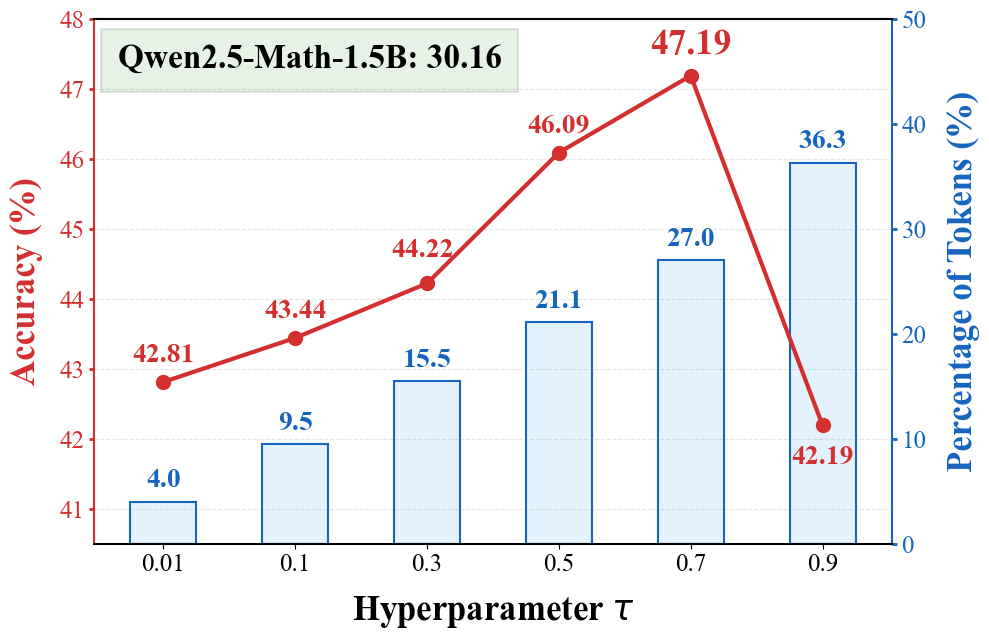
\includegraphics[width=0.5\linewidth]{GFT/Figure/tao.png}
    \caption{Effect of the clipping threshold $\tau$: larger $\tau$ rectifies more tokens. Accuracy follows an inverted U-shape; insufficient clipping is unstable, while excessive clipping reduces learning efficiency.}
    \label{fig:hyper_tau}
\end{figure}

% To identify robust hyperparameter settings on Qwen2.5-Math-1.5B, we ablate the \textbf{group composition ratio} $N_{\mathrm{demo}}:N_{\mathrm{sample}}$ and the \textbf{rectification threshold} $\tau$. \textbf{First}, with fixed group size $K=8$, Table~\ref{tab:hyper_ratio} shows that the \textbf{2:6} setting achieves the best average performance, suggesting that minimal demonstration is sufficient to anchor correctness while more self-sampled trajectories provide stronger within-group contrastive signals for group-advantage learning. \textbf{Second}, sweeping $\tau \in [0.1,0.9]$ exhibits an inverted U-shape in Figure~\ref{fig:hyper_tau}: small $\tau$ ($<0.3$) is too permissive to stabilize updates, whereas large $\tau$ ($>0.8$) over-filters valid tokens and weakens learning; a mid-range $\tau \approx 0.7$ offers the best stability--plasticity trade-off.

To probe the impact of \textbf{group diversity} and \textbf{rectification strength}, we ablate the composition ratio ($N_{\mathrm{demo}}:N_{\mathrm{sample}}$) and threshold $\tau$ on Qwen2.5-Math-1.5B.
With fixed $K=8$, Table~\ref{tab:hyper_ratio} identifies \textbf{2:6} as optimal, where minimal demonstrations \textit{anchor} correctness while abundant self-samples provide richer \textit{contrastive signals} for advantage learning.
Regarding the clipping threshold $\tau$, Figure~\ref{fig:hyper_tau} reports accuracy together with the fraction of DCR-rectified tokens. As $\tau$ increases, the rectification rate rises monotonically, indicating stronger clipping. Meanwhile, accuracy exhibits an \textbf{inverted U-shape}: small $\tau$ yields insufficient clipping and unstable updates, whereas large $\tau$ over-clips many tokens and attenuates informative gradients, harming learning efficiency. Consequently, $\tau \approx 0.7$ achieves the best \textbf{stability--efficiency trade-off} in learning. Notably, GFT consistently outperforms the base model across the entire sweep of parameters, suggesting that DCR is robust to $\tau$.




% \paragraph{Impact of Threshold $\tau$.}
% We vary the DCR threshold $\tau$ from 0.1 to 0.9. Figure \ref{fig:hyper_tau} reveals an inverted U-shape trend. Low thresholds ($\tau < 0.3$) are too lenient to suppress gradient explosion effectively, while overly aggressive thresholds ($\tau > 0.8$) hinder knowledge injection by filtering valid tokens. We find that a mid-range value (e.g., $\tau \approx 0.5$) strikes the optimal balance between stability and plasticity.

\section{Conclusion}
In this work, we analyze SFT as a special case of RL. This perspective reveals two intrinsic limitations: single-path dependency that restricts exploration, and gradient explosion that causes instability. To address these, we propose \textbf{Group Fine-Tuning (GFT)}. This framework leverages Group Advantage Learning to enhance diversity via contrastive supervision and employs Dynamic Coefficient Rectification to stabilize optimization by preventing extreme weight updates. Experiments demonstrate that GFT effectively balances efficient knowledge injection with robust generalization, offering a principled paradigm for post-training.

% \newpage
\section{Limitations}
Despite GFT's effectiveness, we acknowledge three limitations. First, our evaluation focuses on mathematical reasoning with objective correctness; extending GFT to open-ended tasks with subjective rewards requires further exploration. Second, constructing response groups introduces marginal data preparation overhead compared to standard SFT, though this cost is significantly lower than online RL. Third, due to academic resource constraints, our experiments are limited to models up to 8B parameters; validating GFT on 70B+ models remains an important future direction.

\newpage
\section*{Acknowledgments}
This work is supported by the Key R\&D Program of Ningbo under Grant No.2024Z115


% 参考文献和附录


\bibliographystyle{assets/acl_natbib}
\bibliography{paper}

\clearpage
\beginappendix
\section{Derivation: Viewing SFT as a Special Case of On-Policy RL}
\label{sec:proof}

In this appendix, we provide a detailed derivation showing that supervised fine-tuning (SFT) can be interpreted as a special case of reinforcement learning (RL) with a sparse reward function. Specifically, we show that the gradient of the SFT objective can be rewritten as an on-policy expectation under the current policy via importance sampling.

\subsection{SFT Objective and Gradient}

We consider a dataset of expert demonstrations
\(
\mathcal{D} = \{(x, y^*)\}
\),
where \(x\) denotes the input and \(y^*\) is the expert-provided output. The standard SFT objective is defined as the negative log-likelihood:
\begin{equation}
\mathcal{L}_{\mathrm{SFT}}(\theta)
=
-\mathbb{E}_{(x,y^*) \sim \mathcal{D}}
\left[
\log \pi_\theta(y^* \mid x)
\right].
\end{equation}

Taking the gradient with respect to the model parameters \(\theta\), we obtain
\begin{equation}
\nabla_\theta \mathcal{L}_{\mathrm{SFT}}(\theta)
=
-
\mathbb{E}_{(x,y^*) \sim \mathcal{D}}
\left[
\nabla_\theta \log \pi_\theta(y^* \mid x)
\right].
\label{eq:sft_grad_expert}
\end{equation}

This expectation is taken over the expert data distribution rather than samples generated by the current policy.

\subsection{Importance Sampling Reformulation}

We factorize the expert data distribution as
\begin{equation}
P(x, y^*) = P(x)\, P_{\mathrm{expert}}(y^* \mid x),
\end{equation}
and define the joint distribution induced by the current policy as
\begin{equation}
Q(x, y) = P(x)\, \pi_\theta(y \mid x).
\end{equation}

Since both distributions share the same marginal \(P(x)\), we can apply importance sampling to rewrite the expectation in Eq.~\eqref{eq:sft_grad_expert} under \(Q(x,y)\):
\begin{equation}
\begin{aligned}
&\nabla_\theta \mathcal{L}_{\mathrm{SFT}}(\theta)\\
&=
-
\mathbb{E}_{(x,y) \sim Q}
\left[
\nabla_\theta \log \pi_\theta(y \mid x)
\cdot
\frac{P_{\mathrm{expert}}(y \mid x)}{\pi_\theta(y \mid x)}
\right].
\end{aligned}
\label{eq:sft_importance}
\end{equation}

For deterministic expert demonstrations, the expert conditional distribution reduces to a Dirac delta:
\begin{equation}
P_{\mathrm{expert}}(y \mid x) = \mathbb{I}[y = y^*].
\end{equation}

Substituting this into Eq.~\eqref{eq:sft_importance} yields
\begin{equation}
\begin{aligned}
&\nabla_\theta \mathcal{L}_{\mathrm{SFT}}(\theta)\\
&=
-
\mathbb{E}_{(x,y) \sim Q}
\left[
\frac{\mathbb{I}[y = y^*]}{\pi_\theta(y \mid x)}
\nabla_\theta \log \pi_\theta(y \mid x)
\right].
\end{aligned}
\label{eq:sft_final_form_app}
\end{equation}

This recovers the equivalent on-policy formulation presented in the main text.

\subsection{Reinforcement Learning Interpretation}

Equation~\eqref{eq:sft_final_form_app} admits a direct reinforcement learning interpretation. In particular, it corresponds to an on-policy policy gradient with:
\begin{itemize}
    \item \textbf{Policy:} \(\pi_\theta(y \mid x)\);
    \item \textbf{Reward function:}
    \begin{equation}
    r(x,y) = \mathbb{I}[y = y^*],
    \end{equation}
    which provides a unit reward only when the sampled output exactly matches the expert demonstration;
    \item \textbf{Importance weight:}
    \begin{equation}
    w(x,y) = \frac{1}{\pi_\theta(y \mid x)},
    \end{equation}
    correcting for sampling from the model policy instead of the expert distribution.
\end{itemize}

Under this view, SFT can be regarded as a degenerate RL setting with an extremely sparse reward signal and high variance, where learning occurs only through trajectories that coincide exactly with expert demonstrations.

\subsection{Summary}

In summary, the derivation proceeds by (i) expressing the SFT gradient as an expectation over expert data, (ii) applying importance sampling to rewrite it under the model policy, and (iii) specializing the expert distribution to a deterministic form. This establishes a formal equivalence between SFT and on-policy reinforcement learning with a sparse indicator reward, providing a unified perspective on supervised and reinforcement-based post-training.

\section{Formulation of Group Fine-Tuning}
\label{sec:formulation}

In this appendix, we provide the explicit loss formulations and gradient expressions of Group Fine-Tuning (GFT), including both sequence-level and token-level forms. These formulations correspond to the gradient expression presented in Eq.~\eqref{eq:gft_gradient} in the main text.

\subsection{Sequence-Level Objective}
\label{subsec:seq_level_obj}

For each input query \(x\), we construct a response group
\(
\mathcal{G}_x = \{y_1, \ldots, y_K\}
\),
where each response \(y_k\) is assigned a scalar reward \(R(y_k)\) and a standardized
group advantage \(A(y_k)\) as defined in Eq.~\eqref{eq:advantage}. We define the sequence-level GFT loss as
\begin{equation}
\begin{aligned}
\mathcal{L}_{\mathrm{GFT}}^{\mathrm{seq}}(\theta)
=
-
\mathbb{E}_{x}
\Bigg[
\sum_{y_k \in \mathcal{G}_x}
A(y_k)\,
\mathcal{C}\!\left(\pi_\theta(y_k \mid x)\right)
\\[-1mm]
\quad\cdot
\log \pi_\theta(y_k \mid x)
\Bigg].
\end{aligned}
\label{eq:gft_loss_seq}
\end{equation}

where \(\mathcal{C}(\cdot)\) is the dynamic coefficient rectification function defined
in Eq.~\eqref{eq:rectification_factor}.

Taking the gradient of Eq.~\eqref{eq:gft_loss_seq} yields the sequence-level policy gradient:
\begin{equation}
\begin{split}
\nabla_\theta \mathcal{L}_{\mathrm{GFT}}^{\mathrm{seq}}
&= 
\mathbb{E}_{x}
\Bigg[
\sum_{y_k \in \mathcal{G}_x}
A(y_k)\,
\frac{\mathcal{C}\left(\pi_\theta(y_k \mid x)\right)}{\pi_\theta(y_k \mid x)}
\\
&\qquad\cdot 
\nabla_\theta \log \pi_\theta(y_k \mid x)
\Bigg].
\end{split}
\label{eq:gft_grad_seq}
\end{equation}

\subsection{Token-Level Decomposition}
\label{subsec:token_level_decomp}

Each response sequence \(y_k = (y_{k,1}, \ldots, y_{k,T_k})\) is generated autoregressively by the policy:
\begin{equation}
\pi_\theta(y_k \mid x)
=
\prod_{t=1}^{T_k}
\pi_\theta\!\left(y_{k,t} \mid y_{k,<t}, x\right).
\end{equation}

Accordingly, the sequence log-probability decomposes as
\begin{equation}
\log \pi_\theta(y_k \mid x)
=
\sum_{t=1}^{T_k}
\log \pi_\theta\!\left(y_{k,t} \mid y_{k,<t}, x\right).
\end{equation}

We use the shorthand
\begin{equation}
\pi_{k,t}
\triangleq
\pi_\theta\!\left(y_{k,t} \mid y_{k,<t}, x\right).
\label{eq:pi_kt_def}
\end{equation}
for the token-level prediction probability.

Substituting the above decomposition into Eq.~\eqref{eq:gft_loss_seq}, we obtain the token-level GFT loss:
\begin{equation}
\begin{split}
& \mathcal{L}_{\mathrm{GFT}}^{\mathrm{tok}}(\theta)
= % 第一行
\\
& - % 第二行 & 放在最前面，这样就会和第一行的开头对齐（顶格）
\mathbb{E}_{x}
\Bigg[
\sum_{y_k \in \mathcal{G}_x}
A(y_k)\,
\sum_{t=1}^{T_k}
\mathcal{C}(\pi_{k,t})\,
\log \pi_{k,t}
\Bigg].
\end{split}
\label{eq:gft_loss_tok}
\end{equation}

Taking the gradient yields the token-level policy gradient:
\begin{equation}
\begin{split}
& \nabla_\theta \mathcal{L}_{\mathrm{GFT}}^{\mathrm{tok}}
= % 第一行结束在等号
\\
& \mathbb{E}_{x} % & 放在最前面，确保与第一行开头对齐
\Bigg[
\sum_{y_k \in \mathcal{G}_x}
A(y_k)\,
\sum_{t=1}^{T_k}
\frac{\mathcal{C}(\pi_{k,t})}{\pi_{k,t}}\,
\nabla_\theta
\log \pi_{k,t}
\Bigg].
\end{split}
\label{eq:gft_grad_tok}
\end{equation}

\subsection{Relation to SFT and RL Objectives}
\label{subsec:relation_sft_rl}

When the response group degenerates to a single expert demonstration (\(|\mathcal{G}_x| = 1\)), the advantage is constant and Eq.~\eqref{eq:gft_grad_tok} reduces to the standard SFT gradient. Conversely, when the group consists of diverse sampled trajectories with non-trivial advantage values, GFT recovers an on-policy reinforcement learning update with group-normalized advantage weighting and bounded importance coefficients.

This formulation establishes GFT as a strict generalization of SFT and a stabilized, contrastive variant of policy-gradient-based post-training.

% \section{More Experiment}

% \subsection{Main Results on VLLM base model}\label{sec:main_results_VLLM}

% \begin{table*}[t]
%     \centering
%     \small % 稍微减小字号
%     \caption{Main results on Multimodal reasoning benchmarks. We compare GFT with various baselines across different model families. \textbf{Bold} indicates the best performance within each model group. Note that GFT and GRPO use only \textbf{10k} training data, while other methods use \textbf{100k}.}
%     \label{tab:main_results_mllm}
    
%     % 使用 resizebox 强制将表格宽度适应页面宽度 (\textwidth)
%     \resizebox{\textwidth}{!}{%
%         \setlength{\tabcolsep}{3pt} % 稍微减小列间距以适应更多列
%         \renewcommand{\arraystretch}{1.2} % 稍微增加行高
%         % 列数由 9 改为 8 (Model, Method, 6个Benchmark)
%         \begin{tabular}{llcccccc}
%             \toprule
%             \textbf{Model} & \textbf{Method} & \textbf{AMC23} & \textbf{College Math} & \textbf{Gaokao2023En} & \textbf{Math} & \textbf{Minerva Math} & \textbf{TabMWP} \\
%             \midrule
            
%             % 第一组: Qwen2.5-Math-1.5B
%             \multirow{7}{*}{\textbf{Qwen2.5-Math-1.5B}} 
%             & Base Model & 19.38 & - & - & 31.66 & 8.51 & - \\
%             & + SFT & 31.25 & 36.45 & 48.86 & 60.66 & 23.99 & 79.34 \\
%             & + GRPO & 44.84 & 35.58 & 51.80 & 65.97 & 21.17 & 76.94 \\
%             & + ASFT & 43.12 & 29.40 & 47.99 & 60.35 & 15.55 & 65.06 \\
%             & + PSFT & 31.56 & 33.77 & 47.66 & 59.51 & 19.13 & 71.61 \\
%             & + DFT & 36.40 & 38.76 & 52.75 & 64.35 & 23.75 & 82.08 \\
%             \cmidrule(l){2-8} % 横线范围调整为 2-8
%             & \textbf{+ GFT (Ours)} & \textbf{46.09} & \textbf{40.51} & \textbf{58.32} & \textbf{70.50} & \textbf{30.42} & \textbf{85.24} \\
%             \midrule
            
%             % 第二组: Qwen2.5-Math-7B
%             \multirow{7}{*}{\textbf{Qwen2.5-Math-7B}} 
%             & Base Model & - & - & - & - & - & - \\
%             & + SFT & 41.88 & 38.31 & 54.69 & 67.16 & 31.82 & 87.67 \\
%             & + GRPO & 56.09 & 39.81 & 63.47 & 74.52 & 37.22 & 92.36 \\
%             & + ASFT & 52.81 & 40.76 & 61.55 & 74.31 & 32.47 & 89.37 \\
%             & + PSFT & 41.56 & 38.05 & 56.74 & 67.30 & 34.86 & 83.55 \\
%             & + DFT & 51.09 & 39.31 & 57.46 & 70.42 & 35.31 & 86.94 \\
%             \cmidrule(l){2-8}
%             & \textbf{+ GFT (Ours)} & \textbf{59.47} & \textbf{42.06} & \textbf{65.81} & \textbf{77.31} & \textbf{39.86} & \textbf{93.81} \\
%             \midrule
            
%             % 第三组: DeepSeekMath-7B
%             \multirow{6}{*}{\textbf{DeepSeekMath-7B}} 
%             & Base Model & - & - & - & - & - & - \\
%             & + SFT & - & - & - & - & - & - \\
%             & + GRPO & - & - & - & - & - & - \\
%             & + ASFT & - & - & - & - & - & - \\
%             & + PSFT & - & - & - & - & - & - \\
%             & + DFT & - & - & - & - & - & - \\
%             \cmidrule(l){2-8}
%             & \textbf{+ GFT (Ours)} & - & - & - & - & - & - \\
%             \midrule
            
%             % 第四组: LLaMA-3.1-8B
%             \multirow{6}{*}{\textbf{LLaMA-3.1-8B}} 
%             & Base Model & - & - & - & - & - & - \\
%             & + SFT & - & - & - & - & - & - \\
%             & + GRPO & - & - & - & - & - & - \\
%             & + ASFT & - & - & - & - & - & - \\
%             & + PSFT & - & - & - & - & - & - \\
%             & + DFT & - & - & - & - & - & - \\
%             \cmidrule(l){2-8}
%             & \textbf{+ GFT (Ours)} & - & - & - & - & - & - \\
%             \bottomrule
%         \end{tabular}%
%     }
% \end{table*}

% \subsection{Learning Dynamic}\label{moredynamic}

% \subsection{Pass@k Accuracy and Diversity of GFT}\label{morepass}

% \begin{table}[t]
%     \centering
%     % 更新 Caption 中的 k 值为 8, 16 以匹配表格内容
%     \caption{Comparison of Pass@k ($k=8, 16$) performance between Distillation, GRPO and GFT. High Pass@k indicates that the model has learned a diverse and robust distribution of correct reasoning paths.}
%     \label{tab:passk_appendix}
%     \resizebox{\linewidth}{!}{%
%         \renewcommand{\arraystretch}{1.4}
%         \setlength{\tabcolsep}{5pt}
%         \begin{tabular}{c|l|ccccc}
%             \toprule
%             \textbf{Metric} & \textbf{Method} & \textbf{Math500} & \textbf{Minerva} & \textbf{Olympiad} & \textbf{AIME24} & \textbf{AMC23} \\
%             \midrule
%             % Pass@8 Section: multirow 改为 3 行
%             \multirow{3}{*}{Pass@8} 
%             & Distill & 00.00 & 00.00 & 00.00 & 00.00 & 00.00 \\
%             & GRPO & 00.00 & 00.00 & 00.00 & 00.00 & 00.00 \\
%             & \textbf{GFT (Ours)} & \textbf{00.00} & \textbf{00.00} & \textbf{00.00} & \textbf{00.00} & \textbf{00.00} \\
%             \midrule
%             % Pass@16 Section: multirow 改为 3 行
%             \multirow{3}{*}{Pass@16} 
%             & Distill & 00.00 & 00.00 & 00.00 & 00.00 & 00.00 \\
%             & GRPO & 00.00 & 00.00 & 00.00 & 00.00 & 00.00 \\
%             & \textbf{GFT (Ours)} & \textbf{00.00} & \textbf{00.00} & \textbf{00.00} & \textbf{00.00} & \textbf{00.00} \\
%             \bottomrule
%         \end{tabular}%
%     }
% \end{table}

% \subsection{Hyperparameter Analysis}\label{morehyper}

% \section{Training Settings}
% % \paragraph{Training Settings}
% Following DFT~\citep{wu2025generalization}, we utilize the NuminaMath CoT dataset~\citep{numina_math_datasets}, selected for its extensive diversity ranging from high school exercises to international olympiads. For GFT, we construct a hybrid response group of size $K=8$ per query, comprising 1 expert demonstration, 3 teacher distillations from Qwen2.5-Math-72B, and 4 self-generated samples. Similarly, the GRPO baseline is configured to generate 8 outputs per query. To align the total volume of training data across different paradigms, GFT and GRPO utilize a randomly sampled 10k subset (processing 8 trajectories per query), whereas single-trajectory baselines (e.g., SFT, DFT) are trained on a randomly sampled 100k subset.
% \section{Related work}

\section{Evaluation Settings}
\label{sec:eval_settings}
We conduct evaluations on a broad suite of 11 benchmarks: AMC23~\citep{amc2023dataset}, College Math~\citep{hendrycks2020measuring}, Gaokao~\citep{zhang2023evaluating}, Math~\citep{hendrycks2021measuring}, Minerva Math~\citep{lewkowycz2022solving}, TabMWP~\citep{lu2022dynamic}, OlympiadBench~\citep{he-etal-2024-olympiadbench}, Mmlu Stem~\citep{hendrycks2020measuring}, Sat Math~\citep{zhong2024agieval}, Mawps~\citep{koncel2016mawps}, and Svamp~\citep{patel2021nlp}. These benchmarks are carefully selected to cover a wide spectrum of difficulty levels and reasoning types, ensuring a holistic assessment of the model's capabilities. We report the average Pass@1 accuracy across 16 decoding runs (Pass@16 Average) with a sampling temperature of 0.5 and a maximum generation length of 4096 tokens.


% 第一段
\paragraph{Trade-off Between SFT and RL}
Post-training paradigms typically navigate a trade-off between Supervised Fine-Tuning (SFT) and Reinforcement Learning (RL). SFT is widely recognized for its efficiency in knowledge injection and ``cold-starting''~\citep{zhou2023lima, chung2024scaling}; however, it is prone to mechanical memorization and often fails to generalize to out-of-distribution scenarios~\citep{ouyang2022training, bai2022training, chu2025sft, swamy2025all, huan2025does}. Conversely, RL excels at discovering robust strategies and optimizing long-term objectives~\citep{christiano2017deep}, yet it is computationally expensive and struggles to acquire complex reasoning skills from scratch without sufficient guidance~\citep{schulman2017proximal, sheng2025hybridflow, mandlekar2021matters, chen2025empirical}.

% 第二段
\paragraph{The Synergy Dilemma in Hybrid Post-Training}
Standard hybrid approaches (e.g., SFT followed by RL) attempt to combine these complementary strengths but face a severe ``synergy dilemma''~\citep{ouyang2022training, rafailov2023direct}. Recent studies conclude that this conflict arises from the fundamental training dynamics: the overfitting induced by SFT creates a rigid policy that severely constrains the exploration space required for subsequent RL~\citep{chen2025sft}, while simultaneously leading to reasoning pattern mismatches that hinder effective policy alignment~\citep{chen2025synergy}. Although methods like interleaved updates~\citep{liu2025uft} or preference optimization~\citep{rafailov2023direct} offer partial solutions, they remain dependent on external feedback signals. In contrast, our work addresses this dilemma by transforming the rigid imitation objective into a \textbf{Group Advantage Learning} framework, which explicitly preserves solution diversity and the exploration manifold by optimizing contrastive advantages derived from hybrid response groups.

% 第三段
\paragraph{Single-Stage Hybrids: Mixing Imitation and Exploration}
Several recent studies have attempted to unify SFT and RL by balancing imitation and exploration through modified objectives~\citep{yuan2024self}. Single-stage hybrid methods, such as SRFT~\citep{fu2025srft} and UFT~\citep{liu2025uft}, employ dynamic weighting mechanisms, interleaved updates, or dense verification signals~\citep{wang2024math, yu2024ovm} to mix supervised signals with reinforcement objectives. Similarly, frameworks like HybridFlow~\citep{sheng2025hybridflow} explore flexible combinations of offline and online data to bridge the gap. While approaches like CHORD~\citep{zhu2025anchored} introduce anchor-based constraints to maintain stability, a common limitation across these methods is that they often treat SFT and RL as separate components to be linearly combined or alternated, rather than fusing them mathematically into a cohesive formulation derived from a unified training dynamic.

% 第四段
\paragraph{Gradient-Level Stabilization and Its New Trade-offs}
To address the instability inherent in post-training, other researchers have revisited the underlying gradient formulation. Theoretical analyses suggest a deeper equivalence between likelihood maximization and reinforcement learning~\citep{swamy2025all}, prompting new rectification strategies. For instance, \citet{wu2025generalization} propose Dynamic Fine-Tuning (DFT), which counteracts gradient explosion by reweighting the loss with the model's likelihood to cancel the inverse-probability term. However, this indiscriminate dampening creates a new dilemma: it suppresses the strong gradient signals required for injecting novel knowledge, potentially hindering adaptation to new domains. Alternatively, approaches like Proximal SFT~\citep{zhu2025proximal} and Anchored SFT~\citep{zhu2025anchored} introduce trust-region constraints to stabilize fine-tuning, yet such rigid regularizations may overly constrain the model's plasticity. In the realm of Reinforcement Learning, stability is traditionally enforced via KL-divergence penalties~\citep{ouyang2022training} or clipping mechanisms~\citep{schulman2017proximal}. More recently, group-based methods like GRPO~\citep{shao2024deepseekmath} have emerged to mitigate gradient variance by normalizing advantages within generated groups, effectively removing the reliance on unstable critic models, while system-level frameworks like HybridFlow~\citep{sheng2025hybridflow} attempt to stabilize training through flexible data scheduling.


\end{document}